\section{Processi primari}
\subsection{Fornitura}
\subsubsection{Scopo}
Lo scopo della seguente sezione è formalizzare le norme e le procedure che il gruppo \Gruppo{} deve applicare al fine di diventare fornitore del proponente \Proponente{} e dei committenti \VT{} e \CR{}.

\subsubsection{Descrizione} 
Il processo primario di fornitura ha l'obiettivo di capire e comprendere tutte le richieste del proponente, redigendo uno studio di fattibilità. 
Il gruppo \Gruppo{} ha il compito di valutare tali richieste e tenere in considerazione le risorse necessarie ai fini del progetto, esponendo al proponente \Proponente{} le attività che intende svolgere per realizzare il prodotto richiesto.
Tutte queste informazioni vengono inserite nel Piano di Progetto, il quale deve accompagnare il gruppo per tutta la durata del progetto.
Il gruppo \Gruppo{} deve cercare di essere il più possibile in contatto con il proponente per poter comprendere i suoi bisogni.

\subsubsection{Studio di fattibilità}
Il \Responsabile{} ha il compito di convocare tutti i membri del gruppo \Gruppo{} per discutere le varie tematiche riguardanti i capitolati d'appalto disponibili.
Lo \SdF{} viene redatto dagli analisti, i quali devono analizzare il materiale disponibile e inoltre tenere in considerazione anche ciò che è stato discusso nelle riunioni sul tema.\\
Il documento è strutturato in più sezioni, ognuna riguardante un capitolato d'appalto.
Per ogni capitolato verranno trattati i seguenti punti:
\begin{itemize}
\item Titolo del capitolato:
	\begin{itemize}
	\item Nome del capitolato;
	\item Azienda proponente;
	\item Committenti.
	\end{itemize}
\item Descrizione del capitolato:
	\begin{itemize}
	\item Breve riassunto del prodotto da realizzare, secondo le specifiche richieste dal proponente.
	\end{itemize}
\item Prerequisiti e tecnologie coinvolte:
	\begin{itemize}
	\item Elenco delle tecnologie da utilizzare, con eventuali riferimenti per ulteriori approfondimenti o spiegazioni del contesto applicativo;
	\item In alcuni casi l'azienda proponente consiglia l'utilizzo di certe tecnologie.
	\end{itemize}
\item Vincoli:
	\begin{itemize}
	\item Richieste generali, tecniche e/o organizzative da parte dell'azienda proponente.
	\end{itemize}
\item Aspetti positivi:
	\begin{itemize}
	\item Vengono descritti gli aspetti ritenuti positivi dai membri del gruppo \Gruppo{} del capitolato.
	Possono essere considerati aspetti positivi, ad esempio, l'apprendimento di nuove tecnologie e/o linguaggi, disponibilità di contatto e collaborazione offerta dal proponente e documentazione disponibile online riguardante le tecnologie coinvolte.
	\end{itemize}
\item Aspetti critici:
	\begin{itemize}
	\item Vengono descritti gli aspetti ritenuti critici dai membri del gruppo \Gruppo{} del capitolato.
	Possono essere considerati aspetti critici, ad esempio, l'eccessiva mole di tecnologie da apprendere, i requisiti di vincolo da tenere in considerazione e la scarsa presenza di documentazione online riguardante le tecnologie coinvolte.
	\end{itemize}
\item Conclusioni:
	\begin{itemize}
	\item Valutazione finale motivata dai membri del gruppo \Gruppo{} nella quale vengono esposte le ragioni di interesse o disinteresse nella scelta o meno del capitolato.
	\end{itemize}
\end{itemize}
Tutte queste informazioni appena elencate vengono raccolte nel documento interno \glo{\SdF{}}, sottoposto al processo di \glo{verifica{}} da parte dei verificatori.

%inizio parte scritta da \PF
\subsection{Processo di sviluppo}
\subsubsection{Scopo}
Lo scopo del processo di sviluppo è quello di contenere compiti e attività da svolgere, in modo tale da poter fornire al proponente il prodotto finale da lui richiesto.\\
Per una corretta implementazione del prodotto software devono essere svolti i seguenti punti: 
\begin{itemize}
	\item Fissare gli obiettivi di sviluppo;
	\item Fissare i vincoli tecnologici e di design;
	\item Realizzare un prodotto finale che soddisfi tutti i test di \glo{verifica} e validazione i quali devono rispettare quanto definito dal piano di qualità;
	\item Realizzare un prodotto finale conforme ai \glo{requisiti} richiesti dal proponente.
\end{itemize}
\subsubsection{Descrizione}
Il processo di sviluppo è formato da attività e compiti che fanno parte del ciclo di vita del prodotto software, il quale deve soddisfare tutti i \glo{requisiti} indicati nelle specifiche dal proponente per poter essere accettato.		
Il \glo{processo} di sviluppo come detto in precedenza è formato dalle seguenti attività:
\begin{itemize}
	\item \textbf{Analisi dei Requisiti}: Attività in cui si cerca di capire appieno il problema presentato dal cliente ricavando i \glo{requisiti} da soddisfare nella realizzazione del prodotto;
	\item \textbf{Progettazione}: Attività che segue l'analisi dei requisiti nella quale si stabilisce come devono essere realizzati i \glo{requisiti} imposti cliente;
	\item \textbf{Codifica}: Attività in cui si realizza concretamente quello che nel progetto è stato  studiato precedentemente;
	\item \textbf{Test}: Attività in cui si verifica che ogni pezzo di codice scritto durante l'attività di codifica sia privo di errori. Il tutto deve risultare conforme alle aspettative prefissate precedentemente nella way of working;
	\item \textbf{Collaudo}: Attività svolta in concomitanza con il proponente in cui si esegue un test finale che dimostri che il prodotto software realizzato soddisfa tutti i \glo{requisiti} presenti nel capitolato.
\end{itemize}
%fine parte scritta da \PF

\documentclass[a4paper, oneside, dvipsnames, table]{article}
\usepackage{../../Utilita/Stiletemplate}
\usepackage{hyperref}
\usepackage{fancyhdr}
\usepackage[italian]{babel}
\usepackage[raggedright]{titlesec}
\usepackage{blindtext}
\usepackage[export]{adjustbox}
\titleformat{\paragraph}[hang]{\normalfont\normalsize\bfseries}{\theparagraph}{1em}{}
\titlespacing*{\paragraph}{0pt}{3.25ex plus 1ex minus .2ex}{0.5em}

\newcommand{\Titolo}{Piano di Qualifica}

\newcommand{\Redattori}{\AT{} \newline \MC{} \newline \BR{}}

\newcommand{\Verificatori}{\LD{} \newline \DF{}}

\newcommand{\Approvatore}{\SE{}}

\newcommand{\Distribuzione}{\Proponente{} \newline \VT{} \newline \CR{} \newline Gruppo \Gruppo{}}

\newcommand{\Uso}{Esterno}

\newcommand{\DescrizioneDoc}{Questo documento si occupa di descrivere il \PdQ{} realizzato dal Gruppo \Gruppo{} per il progetto \NomeProgetto{}.}

\newcommand{\pathimg}{../../Utilita/Immagini/qbteam.png}

\newcommand{\Versionedoc}{2.0.0}
% scritto da \DF{},\AT{}

% info generali 
\newcommand{\NomeProgetto}{\textit{Stalker}}

% fornitore
\newcommand{\Gruppo}{\textit{qbteam}}
\newcommand{\Mail}{qbteamswe@gmail.com}
% \newcommand{\pathimg}{Immagini/qbteam.png}

% committenti
\newcommand{\Committente}{\VT \newline \CR}
\newcommand{\VT}{Prof. Vardanega Tullio}
\newcommand{\CR}{Prof. Cardin Riccardo}

% proponenti
\newcommand{\Proponente}{\textit{Imola Informatica}}
\newcommand{\ZD}{Zanetti Davide}
\newcommand{\CT}{Cardona Tommaso}

% qbteam
\newcommand{\AT}{Azzalin Tommaso}
\newcommand{\DF}{Drago Francesco}
\newcommand{\BR}{Baratin Riccardo}
\newcommand{\MC}{Mattei Christian}
\newcommand{\PF}{Perin Federico}
\newcommand{\CE}{Cisotto Emanuele}
\newcommand{\SE}{Salmaso Enrico}
\newcommand{\LD}{Lazzaro Davide}

% ruoli
\newcommand{\Responsabile}{Responsabile di Progetto}
\newcommand{\Amministratore}{Amministratore di Progetto}

% documenti

\newcommand{\SdF}{Studio di Fattibilità}
\newcommand{\SdFv}[1]{\textit{Studio di Fattibilità {#1}}}
\newcommand{\PdQ}{Piano di Qualifica}
\newcommand{\PdQv}[1]{\textit{Piano di Qualifica {#1}}}
\newcommand{\PdP}{Piano di Progetto}
\newcommand{\PdPv}[1]{\textit{Piano di Progetto {#1}}}
\newcommand{\NdP}{Norme di Progetto}
\newcommand{\NdPv}[1]{\textit{Norme di Progetto {#1}}}
\newcommand{\AdR}{Analisi dei Requisiti}
\newcommand{\AdRv}[1]{\textit{Analisi dei Requisiti {#1}}}
\newcommand{\Glossario}{Glossario}
\newcommand{\Glossariov}[1]{\textit{Glossario {#1}}}
\newcommand{\MM}{Manuale Manutentore}
\newcommand{\MU}{Manuale Utente}

% comandi generali
\newcommand{\glo}[1]{#1\ap{G}}

\setlength{\parindent}{-0.1em}


\begin{document}

\copertina{}
\newpage

\section*{Registro delle modifiche}
{
\rowcolors{2}{grigetto}{white}
\renewcommand{\arraystretch}{1.5}
\centering
\begin{longtable}{ c c  C{2.3cm} c C{3cm} C{3.2cm}}
\rowcolor{rossoep}
\textcolor{white}{\textbf{Versione}} & \textcolor{white}{\textbf{Data}} & \textcolor{white}{\textbf{Nominativo}} & \textcolor{white}{\textbf{Ruolo}} & 
\textcolor{white}{\textbf{Verificatore}}& \textcolor{white}{\textbf{Descrizione}}\\	


1.0.0 & \Data & \CE{} & Responsabili & \CE{} & Approvazione per il rilascio.  \\
		
0.0.1 & \Data & \DF{} & Analista & \AT{} & Stesura e verifica del documento.  \\
		
		
\end{longtable}
}

\fancydoc{}

\clearpage
\tableofcontents
\clearpage
\listoffigures
\clearpage

% scritto da\AT{}
\section{Introduzione}
\subsection{Scopo del documento}
Il presente documento ha lo scopo di descrivere le strategie che il gruppo \Gruppo{} intende applicare per garantire la qualità di processo e di prodotto per l’intera durata del progetto.
Al fine di rispettare questi obiettivi vengono descritte le modalità in cui vengono effettuate la verifica e la validazione del prodotto.
In questo modo è consentita la rilevazione e correzione di problemi o incongruenze in breve tempo, senza correre il rischio di sprechi di risorse.

\subsection{Scopo generale del prodotto}
L'obiettivo del prodotto \NomeProgetto{} di \Proponente{} è la creazione di un sistema software composto di un applicativo per cellulare e di un server, con cui interagire tramite un'interfaccia utente. La necessità nasce dal bisogno di adempiere alle normative vigenti in tema di sicurezza.
Le due componenti del sistema software, applicativo e server, devono soddisfare i seguenti obiettivi rispettivamente di:
\begin{itemize}
\item Tracciare e registrare i \glo{movimenti} di un utente in un \glo{luogo di tracciamento} di un'\glo{organizzazione}, siano essi autenticati da credenziali di un'\glo{organizzazione} oppure visitatori anonimi, il tutto nel rispetto della normativa sulla privacy;
\item Poter visionare gli accessi degli utenti autenticati e visionare il numero di visitatori anonimi all'interno di un luogo.
\end{itemize}

\subsection{Glossario}
Al fine di evitare ambiguità fra i termini, e per avere chiare fra tutti gli stakeholder le terminologie utilizzate per la realizzazione del presente documento, il gruppo \Gruppo{} ha redatto un documento denominato \Glossariov{1.0.0}.
In tale documento, sono presenti tutti i termini tecnici, ambigui, specifici del progetto e scelti dai membri del gruppo con le loro relative definizioni.
Un termine presente nel \Glossariov{1.0.0} e utilizzato in questo documento viene indicato con un apice \ap{G} alla fine della parola.

\subsection{Standard di progetto}
Il gruppo \Gruppo{} ha deciso di gestire i propri processi del ciclo di vita del software adottando alcune parti dello standard \textbf{ISO/IEC 12207} come definito nelle \textit{NormeDiProgetto}; 
come modello di qualità del prodotto software si è utilizzato parte dello standard \textbf{ISO/IEC 9126} anch'esso definito nelle \textit{NormeDiProgetto}.

\subsection{Riferimenti}

\subsubsection{Normativi}
\begin{itemize}
    \item \textbf{Capitolato d'appalto C5 - Stalker}\\     
    \url{https://www.math.unipd.it/~tullio/IS-1/2019/Progetto/C5.pdf};
    \item \NdPv{1.0.0}.
    \item \textbf{ISO/IEC 12207-1995:}\\     
    \url{https://www.math.unipd.it/~tullio/IS-1/2009/Approfondimenti/ISO_12207-1995.pdf};\\
    \url{http://www.colonese.it/SviluppoSw_Standard_ISO12207.html};
    \item \textbf{ISO/IEC 9126:}\\
    \url{http://www.colonese.it/00-Manuali_Pubblicatii/07-ISO-IEC9126_v2.pdf};\\
    \url{https://en.wikipedia.org/wiki/ISO/IEC_9126};
\end{itemize}

\subsubsection{Informativi}
\begin{itemize}
    \item \textbf{Indice di Gulpease}\\
    \url{https://it.wikipedia.org/wiki/Indice_Gulpease};
    \item \textbf{Metriche di progetto}\\
    \url{https://it.wikipedia.org/wiki/Metriche_di_progetto};
    \item \textbf{Varie metriche}\\
    \url{http://torlone.dia.uniroma3.it/sistelab/annipassati/sbavaglia.pdf};
    \item \textbf{Ciclo di Deming - Plan Do Check Act}\\
    \url{https://it.wikipedia.org/wiki/Ciclo_di_Deming};
    
\end{itemize}

\section{Descrizione generale}
\subsection{Contesto d'uso del prodotto}
Il prodotto è orientato ai seguenti utenti: proprietari di \glo{organizzazioni} per la sezione della web app, mentre l'app sarà orientata a visitatori e clienti di \glo{organizzazioni} pubbliche e dipendenti di \glo{organizzazioni} private.
Il prodotto servirà per tracciare gli utenti dell'applicazione al fine di rispettare le norme vigenti sulla sicurezza nei luoghi pubblici oppure per agevolare la gestione e la tracciabilità dei dipendenti dell'azienda.
Alcune funzionalità del prodotto, come la creazione di un'\glo{organizzazione} e la sua eliminazione non verranno eseguite dagli utenti a cui è rivolto lo stesso. Sarà compito degli amministratori del sistema \NomeProgetto{} occuparsene, che non rientrano tra gli attori del prodotto.

\subsection{Funzioni del prodotto}
Il prodotto garantirà le seguenti funzionalità:
\begin{itemize}
    \item \textbf{Amministratori:} gli amministratori dovranno essere in grado, attraverso la web app, di gestire la propria \glo{organizzazione}, visualizzare gli accessi dei dipendenti e nominare altri amministratori per assisterli nella gestione e monitoraggio. \\
        L'amministratore avrà accesso alle seguenti funzionalità:
        \begin{itemize}
            \item \textbf{Modifica ai parametri dell'\glo{organizzazione}}: L'amministratore può ridefinire il nome, la descrizione, l'immagine e l'indirizzo dell'\glo{organizzazione} selezionata;
            \item \textbf{Modifica delle superfici geografiche di \glo{tracciamento} dell'\glo{organizzazione}}: Può modificare il perimetro di \glo{tracciamento} dell'\glo{organizzazione} e quello degli specifici \glo{luoghi}, inserendo un numero a piacere di coordinate per delimitarne la superficie di \glo{tracciamento} (manualmente o tramite Google Maps API);
            \item \textbf{Gestione degli amministratori}: È possibile nominare e/o eliminare amministratori e modificarne i privilegi;
            \item \textbf{Monitoraggio degli utenti tracciati}: L'amministratore può sapere, in tempo reale, quanti utenti si trovano all'interno dei vari \glo{luoghi} dell'\glo{organizzazione}, o dell'organizzazione in generale. Qualora l'\glo{organizzazione} monitorata fosse gestita con tracciamento riconosciuto, l'amministratore è anche in grado di sapere l'identità dei vari utenti tracciati;
            \item \textbf{Visualizzazione degli accessi effettuati}: L'amministratore ha la possibilità di visualizzare lo storico degli accessi degli utenti che hanno effettuato l'accesso all'\glo{organizzazione}, qualora quest'ultima fosse monitorata con tracciamento riconosciuto. Per ogni accesso di uno specifico utente viene mostrato: il timestamp di ingresso, quello di uscita e il suo tempo di permanenza presso l'organizzazione.
            \item \textbf{Estrapolazione di report tabellari riguardanti gli accessi dei dipendenti e gli accesi ai vari luoghi dell'\glo{organizzazione}}: L'amministratore può ricavare tabelle dei seguenti tipi:
            \begin{itemize}
                \item ore di entrata e uscita da un luogo per uno specifico utente;
                \item totale di ore spese in ogni luogo per uno specifico utente;
                \item il numero di dipendenti e il totale delle ore da loro trascorse in ogni luogo dell'\glo{organizzazione}.
            \end{itemize}
        \end{itemize}
    \item \textbf{Utenti:} gli utenti necessiteranno della possibilità, con l'applicazione, di registrarsi e autenticarsi nell'app, di venire tracciati nelle \glo{organizzazioni} e autenticarsi presso le \glo{organizzazioni} che lo richiedono. Agli utenti saranno fornite le seguenti funzionalità:
    \begin{itemize}
        \item \textbf{Funzionalità di registrazione e \glo{autenticazione}}: L'utente può registrarsi con delle nuove credenziali o, alternativamente, effettuare l'accesso con un account già registrato nel sistema. Qualora l'utente avesse smarrito la password, avrebbe comunque la possibilità di effettuarne il reset;
        \item \textbf{Possibilità di scaricare e aggiornare la lista delle \glo{organizzazioni}}: L'utente ha la possibilità di scaricare la lista delle organizzazioni, sia quelle con \glo{tracciamento} autenticato che quelle senza. Può inoltre effettuare l'aggiornamento della lista in maniera manuale, tramite un pulsante o temporizzata;
        \item \textbf{Venire tracciati nelle \glo{organizzazioni} desiderate}: L'utente verrà tracciato qualora effettuasse un \glo{movimento} all'interno dell'\glo{organizzazione};
        \item \textbf{Gestione delle \glo{organizzazioni} preferite}: L'utente può selezionare un'organizzazione e renderla preferita, così facendo essa sarà visualizzata nelle prime righe della lista delle organizzazioni;
        \item \textbf{Visualizzare gli accessi effettuati presso le varie \glo{organizzazioni} e i relativi luoghi}: L'utente ha a disposizione un registro degli accessi in cui sarà visualizzato l'orario di entrata e uscita da una determinata organizzazione, o luogo, e il tempo trascorso al suo interno;
        \item \textbf{Passare in tracciabilità anonima e non presso \glo{organizzazioni} private}: Un utente riconosciuto potrà decidere di passare all'anonimato, cioè di diventare un utente anonimo, selezionando l'apposita funzionalità.
    \end{itemize}
\end{itemize}
\subsection{Vincoli generali}
Per gli amministratori è sufficiente un browser (su di un computer con connessione ad internet); per gli utenti dell'applicazione un dispositivo con SO Android, una connessione a internet e/o un modulo GPS.

\section{Casi d'uso}
\subsection{Attori}
\subsubsection{Attori Utenti}

\begin{figure}[h]
  \centering
    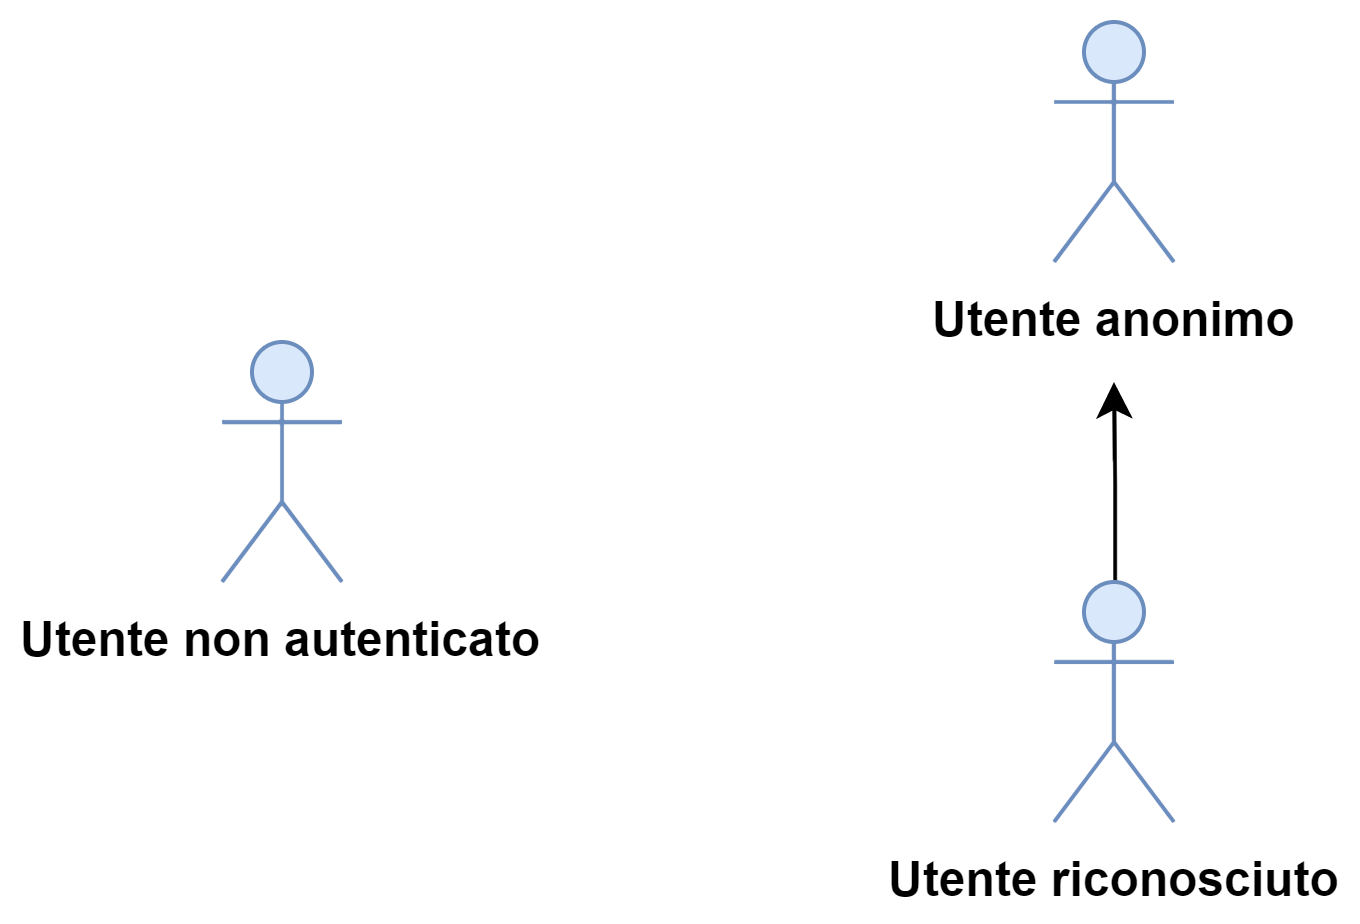
\includegraphics[scale=0.8]{Sezioni/UseCase/Immagini/Utenti.png}
    \caption{Gerarchia degli utenti}
\end{figure}

\paragraph{Utente non autenticato}
Utente non ancora autenticato all'applicazione che può avere o non avere le credenziali per autenticarsi.
\paragraph{Utente anonimo}
Utente autenticato che può venire tracciato all'interno di una \glo{organizzazione} senza fornire dettagli sulla propria identità.
\paragraph{Utente riconosciuto}
Utente autenticato che è attualmente tracciato all'interno di una precisa \glo{organizzazione} fornendo dettagli sulla propria identità.
L'utente si è precedentemente autenticato presso l'\glo{organizzazione} tramite LDAP.



\subsubsection{Attori Amministratori}
\begin{figure}[h]
  \centering
    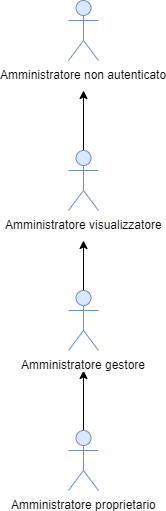
\includegraphics[scale=0.8]{Sezioni/UseCase/Immagini/Amministratori.png}
    \caption{Gerarchia degli amministratori}
\end{figure}


\paragraph{Amministratore non autenticato}
Amministratore non ancora autenticato nel sistema che ha già le credenziali per autenticarsi.
\paragraph{Amministratore autenticato}
Amministratore che si è autenticato nel sistema.
\paragraph{Amministratore proprietario}
Amministratore autenticatosi con il ruolo di proprietario dell'\glo{organizzazione}.
Si trova al gradino più alto della gerarchia degli amministratori e dispone delle seguenti funzioni:
\begin{itemize}
\item Gestire l'\glo{organizzazione}, ovvero modificarne i dati (come nome, descrizione, ecc.) e le superfici geografiche per il \glo{tracciamento} degli utenti;
\item Gestire gli amministratori, cioè la loro nomina, rimozione e modifica dei privilegi;
\item Monitorare gli accessi;
\item Eliminare l'\glo{organizzazione}.
\end{itemize}
Il proprietario dell'\glo{organizzazione} può nominare altri amministratori.
\paragraph{Amministratore gestore}
Amministratore autenticatosi con il ruolo di gestore. 
Si trova al secondo gradino della gerarchia degli amministratori e dispone delle seguenti funzioni:
\begin{itemize}
\item Gestire l'\glo{organizzazione};
\item Monitorare gli accessi.
\end{itemize}
\paragraph{Amministratore visualizzatore}
Amministratore autenticatosi con il ruolo di visualizzatore.
Escludendo l'amministratore non autenticato si trova all'ultimo gradino della gerarchia degli amministratori e può compiere solo la seguente funzione:
\begin{itemize}
\item Monitorare gli accessi.
\end{itemize}

%Alternativa in caso esista una gerarchia a 3 livelli




\clearpage
\subsection{Elenco casi d'uso}
\setcounter{secnumdepth}{0}
\subsubsection{UCA 1 - Accesso all'applicazione}%kite level

\begin{figure}[h]
  \centering
    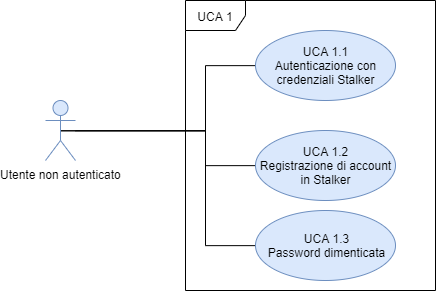
\includegraphics[scale=0.5]{Sezioni/UseCase/Immagini/UCA1.png}
  \caption{UCA 1 - Accesso all'applicazione}
\end{figure}

\begin{itemize}
\item \textbf{Attori primari:} Utente non autenticato
\item \textbf{Precondizione:} L'utente non è autenticato.
\item \textbf{Postcondizione:} L'utente viene autenticato all'interno del sistema tramite registrazione [UCA 1.2] oppure tramite \glo{autenticazione} [UCA 1.1].
\item \textbf{Scenario principale:} L'utente non identificato può scegliere se registrarsi [UCA 1.2] nel sistema oppure, se possiede già un account, accedere [UCA 1.1] all'applicazione. %cosa potrebbe fare l'utente con il UC, descrizione
\end{itemize}

\subsubsection{UCA 1.1 - Autenticazione con credenziali Stalker}%sea level

\begin{figure}[h]
  \centering
    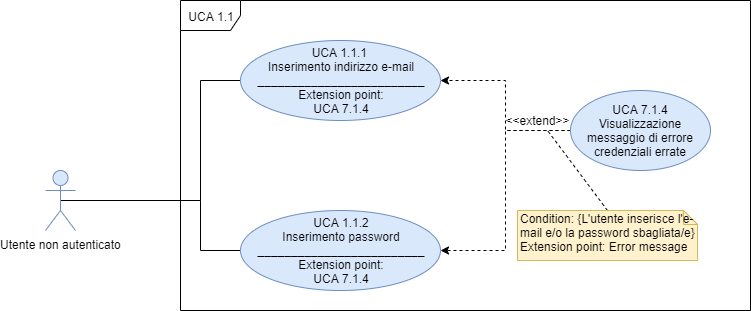
\includegraphics[scale=0.5, center]{Sezioni/UseCase/Immagini/UCA1.1.png}
  \caption{UCA 1.1 - \glo{Autenticazione} con credenziali Stalker}
\end{figure}

\begin{itemize}
\item \textbf{Attori primari:} Utente non autenticato
\item \textbf{Precondizione:} L'utente non è autenticato.
\item \textbf{Postcondizione:} L'utente viene autenticato all'interno del sistema e accede all'applicazione.
\item \textbf{Scenario principale:} L'utente non autenticato inserisce l'indirizzo e-mail e la password per autenticarsi attraverso il modulo di \glo{login} presente.
\item \textbf{Scenario alternativo 1:} L'utente tenta di accedere con delle credenziali errate [UCA 8.1.4].
%\item \textbf{Scenario alternativo 2:} Se l'utente non dovesse ricordarsi la password ha la possibilità di selezionare la funzionalità password dimenticata [UCA 1.3] per reimpostarla.
\item \textbf{Flusso di eventi:}
  \begin{enumerate}
        \item Inserimento indirizzo e-mail [UCA 1.1.1];
        \item Inserimento password [UCA 1.1.2].
    \end{enumerate}
\item \textbf{Estensioni:}
	\begin{itemize}
		\item UCA 8.1.4 - Visualizzazione messaggio di errore credenziali errate;
	\end{itemize}
%\item \textbf{Inclusioni:}
\end{itemize}

\subsubsection{UCA 1.1.1 - Inserimento indirizzo e-mail}%fish level
\begin{itemize}
\item \textbf{Attori primari:} Utente non autenticato
\item \textbf{Precondizione:} L'utente non è autenticato.
\item \textbf{Postcondizione:} L'utente ha inserito il proprio indirizzo e-mail.
\item \textbf{Scenario principale:} Inserimento indirizzo e-mail per l'autenticazione.
\end{itemize}

\subsubsection{UCA 1.1.2 - Inserimento password}%fish level
\begin{itemize}
\item \textbf{Attori primari:} Utente non autenticato
\item \textbf{Precondizione:} L'utente non è autenticato.
\item \textbf{Postcondizione:} L'utente ha inserito la propria password.
\item \textbf{Scenario principale:} Inserimento password per l'autenticazione.
\end{itemize}

\subsubsection{UCA 1.2 - Registrazione di account in Stalker}%sea level

\begin{figure}[h]
  \centering
    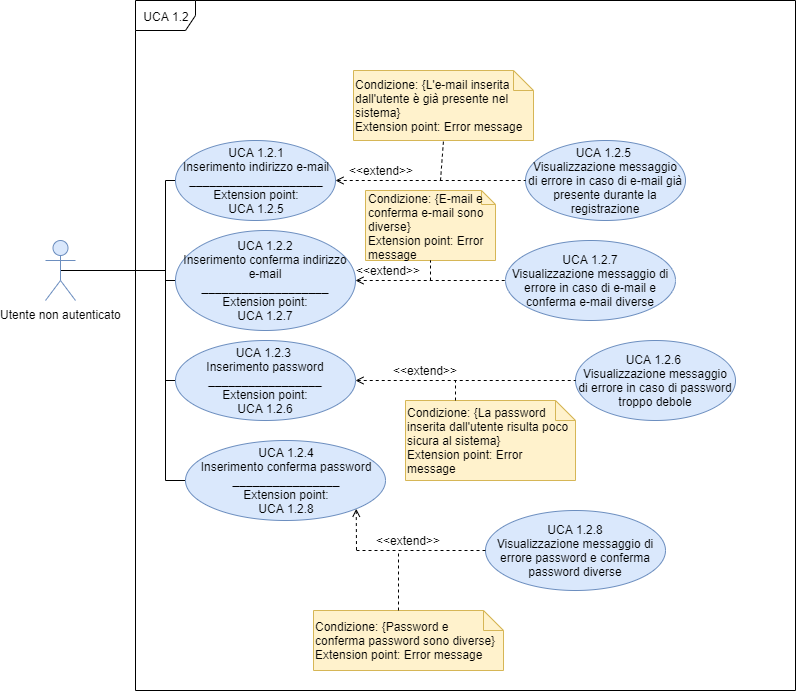
\includegraphics[scale=0.4, center]{Sezioni/UseCase/Immagini/UCA1.2.png}
  \caption{UCA 1.2 -  Registrazione di account in Stalker}
\end{figure}

\begin{itemize}
\item \textbf{Attori primari:} Utente non autenticato
\item \textbf{Precondizione:} L'utente non è ancora registrato nel sistema.
\item \textbf{Postcondizione:} L'utente si è registrato e accede al sistema.
\item \textbf{Scenario principale:} L'utente non registrato compila il modulo di registrazione al fine di poter accedere al sistema.
\item \textbf{Flusso di eventi:}
  \begin{enumerate}
        \item Inserimento indirizzo e-mail [UCA 1.2.1];
        \item Inserimento password [UCA 1.2.2];
        \item Inserimento conferma password [UCA 1.2.3];
        \item Accettazione delle condizioni generali d'uso [UCA 1.2.4];
    \end{enumerate}
\end{itemize}

\subsubsection{UCA 1.2.1 - Inserimento indirizzo e-mail}%fish level

\begin{itemize}
\item \textbf{Attori primari:} Utente non autenticato
\item \textbf{Precondizione:} L'utente non è registrato.
\item \textbf{Postcondizione:} L'utente ha inserito il proprio indirizzo e-mail, di cui è stata verificata la non esistenza in associazione ad altri account nel sistema.
\item \textbf{Scenario principale:} Inserimento indirizzo e-mail per la registrazione.
\item \textbf{Estensioni:}
	\begin{itemize}
		\item UCA 8.1.1 - Visualizzazione messaggio di errore in caso di account con l'e-mail inserita già presente.
	\end{itemize}
\end{itemize}

\subsubsection{UCA 1.2.2 - Inserimento password}%fish level
\begin{itemize}
\item \textbf{Attori primari:} Utente non autenticato
\item \textbf{Precondizione:} L'utente non è registrato.
\item \textbf{Postcondizione:} L'utente ha inserito una password che rispetta i criteri di complessità definiti dal sistema.
\item \textbf{Scenario principale:} Inserimento password per la registrazione.
\item \textbf{Estensioni:}
	\begin{itemize}
		\item UCA 8.1.2 - Visualizzazione messaggio di errore in caso di password troppo debole.
	\end{itemize}
\end{itemize}

\subsubsection{UCA 1.2.3 - Inserimento conferma password}%fish level
\begin{itemize}
\item \textbf{Attori primari:} Utente non autenticato
\item \textbf{Precondizione:} L'utente non è registrato.
\item \textbf{Postcondizione:} L'utente ha confermato la password inserendola nuovamente (è uguale a quella inserita durante l'inserimento della password [UCA 1.2.2]).
\item \textbf{Scenario principale:} Inserimento conferma password.
\item \textbf{Estensioni:}
	\begin{itemize}
		\item UCA 8.1.3 - Visualizzazione messaggio di errore in caso di password e conferma password diverse.
	\end{itemize}
\end{itemize}

\subsubsection{UCA 1.2.4 - Accettazione delle condizioni generali d'uso}%fish level
\begin{itemize}
\item \textbf{Attori primari:} Utente non autenticato
\item \textbf{Precondizione:} L'utente non è registrato.
\item \textbf{Postcondizione:} L'utente ha accettato le condizioni generali sull'uso.
\item \textbf{Scenario principale:} Accettazione delle condizioni generali d'uso.
\item \textbf{Scenario alternativo:} Se l'utente dovesse rifiutare le condizioni generali sull'uso allora la registrazione verrebbe interrotta e l'applicazione chiusa.
\end{itemize}

\begin{figure}[h]
	\centering
	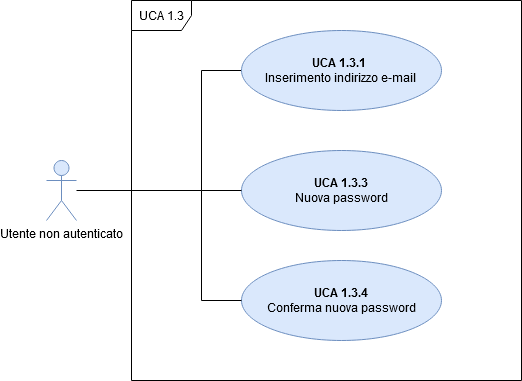
\includegraphics[scale=0.6]{Sezioni/UseCase/Immagini/UCA1.3.png}
	\caption{UCA 1.3 - Password dimenticata}
\end{figure}

\subsubsection{UCA 1.3 - Password dimenticata}%fish level
\begin{itemize}
\item \textbf{Attori primari:} Utente non autenticato
\item \textbf{Precondizione:}  L'utente non è autenticato.
\item \textbf{Postcondizione:} L'utente ha fatto richiesta per avviare la procedura di password dimenticata.
\item \textbf{Scenario principale:} La password è stata dimenticata.
\item \textbf{Flusso di eventi:}
  \begin{enumerate}
        \item Inserimento dell'indirizzo e-mail a cui inviare la e-mail per il cambio password [UCA 1.3.1];
        \item Il sistema invia la e-mail per il cambio password;
        \item Inserimento della nuova password [UCA 1.3.3];
        \item Inserimento della conferma della nuova password [UCA 1.3.4].
    \end{enumerate}
\end{itemize}

\subsubsection{UCA 1.3.1 - Inserimento e-mail}
\begin{itemize}
\item \textbf{Attori primari:} Utente non autenticato
\item \textbf{Precondizione:} L'utente non è autenticato.
\item \textbf{Postcondizione:} L'utente ha inserito l'e-mail.
\item \textbf{Scenario principale:} Inserimento indirizzo e-mail per cambiare password.
\end{itemize}


\subsubsection{UCA 1.3.3 - Nuova password}
\begin{itemize}
\item \textbf{Attori primari:} Utente non autenticato
\item \textbf{Precondizione:}  L'utente non è autenticato.
\item \textbf{Postcondizione:} L'utente inserisce la nuova password.
\item \textbf{Scenario principale:} Inserimento della nuova password.
\end{itemize}

\subsubsection{UCA 1.3.4 - Conferma nuova password}
\begin{itemize}
\item \textbf{Attori primari:} Utente non autenticato
\item \textbf{Precondizione:} L'utente non è autenticato.
\item \textbf{Postcondizione:} L'utente reinserisce la nuova password per confermarla.
\item \textbf{Scenario principale:} Inserimento della conferma della nuova password.
\end{itemize}
\newpage
\subsubsection{UCA 2 - Logout dell'utente dall'applicazione}%kite level
\begin{itemize}
\item \textbf{Attori primari:} Utente autenticato;
\item \textbf{Precondizione:} L'utente si è già autenticato nel sistema e si trova all'interno dell'applicazione;
\item \textbf{Postcondizione:}  L'utente si è disconnesso dal proprio account e non è più autenticato nell'applicazione;
\item \textbf{Scenario principale:} L'utente ha fatto richiesta di avviare la procedura di logout dall'applicazione.
\end{itemize}
%scritto da \PF{}
\subsubsection{UCA 3 - Gestione lista delle organizzazioni}%kite level
\begin{figure}[h]
	\centering
	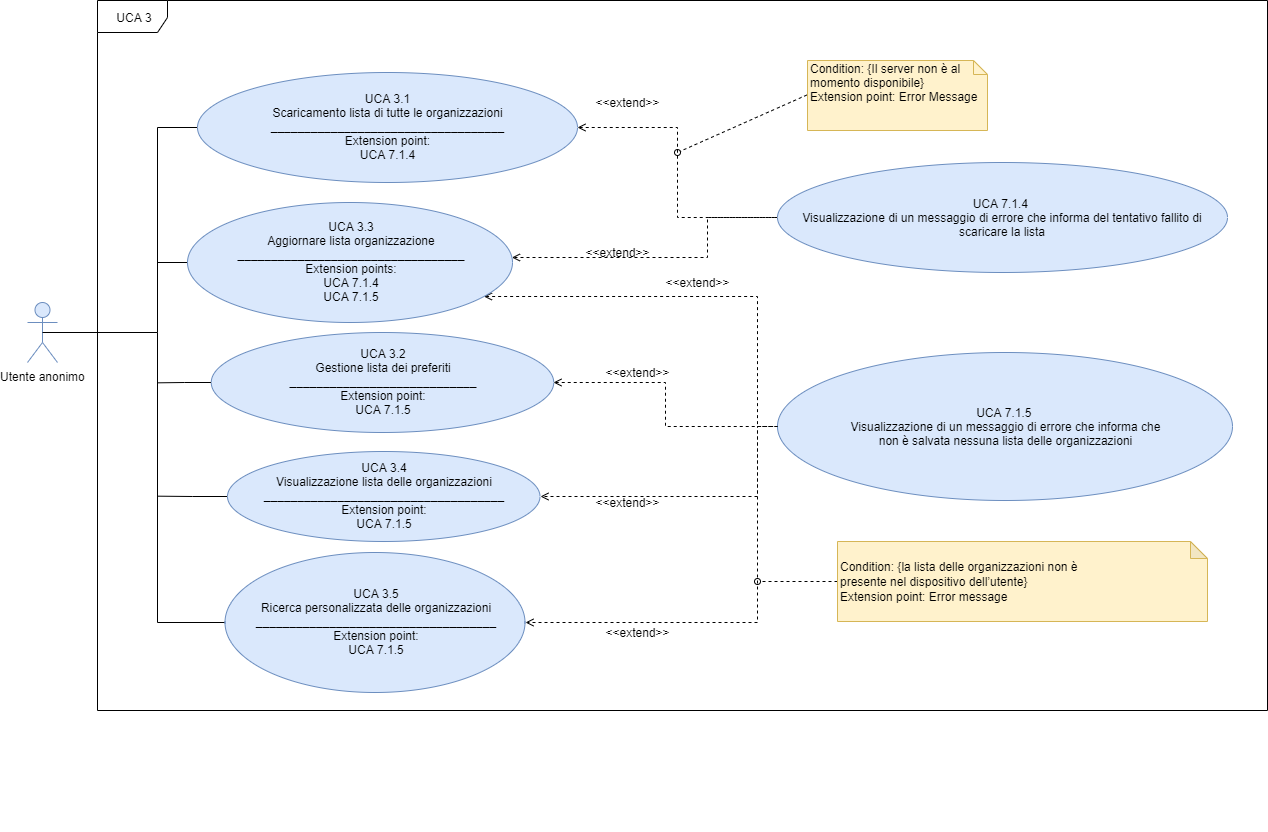
\includegraphics[scale=0.5, center]{Sezioni/UseCase/Immagini/UCA3.png}
	\caption{UCA 3 - Gestione lista delle \glo{organizzazioni}}
\end{figure} 

\begin{itemize}
\item \textbf{Attori primari:} Utente anonimo, Utente riconosciuto
\item \textbf{Precondizione:} L'utente è autenticato e può accedere alle funzionalità della lista delle \glo{organizzazioni}.
\item \textbf{Postcondizione:} Vengono forniti all'utente i risultati delle funzionalità disponibili.
\item \textbf{Scenario principale:} L'utente autenticato utilizza le funzioni di gestione delle liste di \glo{organizzazioni} per svolgere una o più delle seguenti azioni:
	\begin{itemize}
		\item Scaricamento lista di tutte le \glo{organizzazioni} [UCA 3.1];
		\item Gestione lista delle \glo{organizzazioni preferite} [UCA 3.2];
		\item Aggiornare lista \glo{organizzazione} [UCA 3.3];
		\item Visualizzazione lista delle \glo{organizzazioni} [UCA 3.4];
		\item Ricerca personalizzata delle \glo{organizzazioni} [UCA 3.5].
	\end{itemize}
\end{itemize}

\subsubsection{UCA 3.1 - Scaricamento lista di tutte le organizzazioni}%sea level
\begin{itemize}
\item \textbf{Attori primari:} Utente anonimo, Utente riconosciuto
\item \textbf{Precondizione:} L'utente è autenticato e può scaricare la lista di tutte le \glo{organizzazioni}.
\item \textbf{Postcondizione:} L'utente ha a disposizione la lista di tutte le \glo{organizzazioni}.
\item \textbf{Scenario principale:} L'utente seleziona l'esecuzione della funzione "Scaricamento della lista".
\item \textbf{Scenario alternativo:} Se il tentativo di scaricare la lista fallisce viene visualizzato all'utente un messaggio di errore che lo informa di tale problema [UCA 8.3.1].
\item \textbf{Estensioni:}
	\begin{itemize}
	\item UCA 8.3.1 - Visualizzazione di un messaggio di errore che informa del tentativo fallito di scaricare la lista.
\end{itemize}
  
\end{itemize}

\subsubsection{UCA 3.2 - Gestione lista delle organizzazioni preferite}%sea level
\begin{figure}[h]
	\centering
	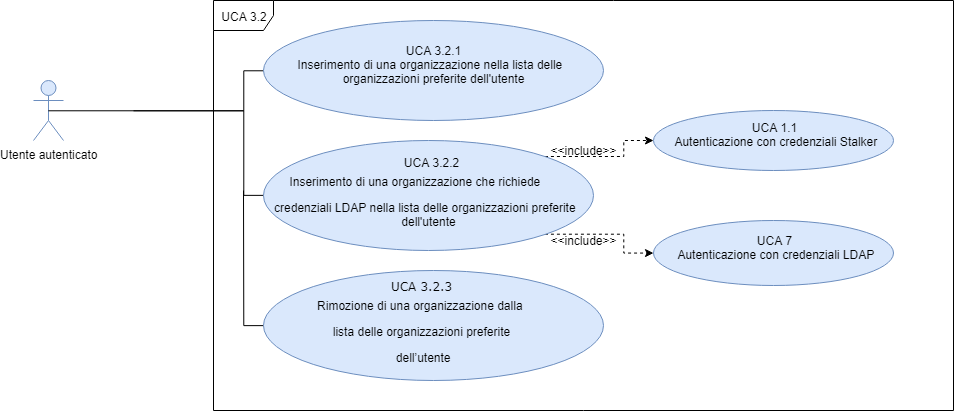
\includegraphics[scale=0.45 , center]{Sezioni/UseCase/Immagini/UCA3.2.png}
	\caption{UCA 3.2 - Gestione lista delle \glo{organizzazioni preferite}}
\end{figure}
\begin{itemize}
	\item \textbf{Attori primari:} Utente anonimo, Utente riconosciuto
	\item \textbf{Precondizione:} L'utente è autenticato e può gestire la propria lista delle \glo{organizzazioni preferite}.
	\item \textbf{Postcondizione:} All'utente vengono forniti i risultati delle funzionalità disponibili.
	\item \textbf{Scenario principale:} L'utente autenticato ha selezionato la funzionalità di gestione della lista delle \glo{organizzazioni preferite}.
	\item \textbf{Flusso di eventi:}
			\begin{enumerate}
			\item L'utente accede alla funzionalità di "Gestioni della lista delle \glo{organizzazioni preferite}";
			\item Vi è la possibilità di inserire un'\glo{organizzazione} nella lista delle \glo{organizzazioni preferite} dell'utente dell'applicazione [UCA 3.2.1], se però viene richiesto di inserire una \glo{organizzazione} che richiede di autenticarsi con credenziali \glo{LDAP} [UCA 3.2.2] allora l'utente dovrà inserire tali credenziali [UCA 1.1];
			\item Vi è la possibilità di rimuovere un'\glo{organizzazione} dalla lista delle \glo{organizzazioni preferite} dell'utente dell'applicazione [UCA 3.2.3].
			\end{enumerate}
	\item \textbf{Scenario alternativo:} Se non è presente nessuna lista delle \glo{organizzazioni} viene visualizzato all'utente un messaggio di errore che lo informa di tale problema [UCA 8.3.2];
	\item \textbf{Estensioni:}
	\begin{itemize}
		\item UCA 8.3.2 - Visualizzazione di un messaggio di errore che informa che non è salvata nessuna lista delle \glo{organizzazioni}.
	\end{itemize}
\end{itemize}

\subsubsection{UCA 3.2.1 - Inserimento di una organizzazione nella lista delle organizzazioni preferite dell'utente}%fish level
\begin{itemize}
	\item \textbf{Attori primari:} Utente anonimo, Utente riconosciuto
	\item \textbf{Precondizione:} L'utente è autenticato sceglie di eseguire la funzionalità di inserimento di un'\glo{organizzazione} nella lista delle \glo{organizzazioni preferite} (solo se ha scaricato precedentemente la lista delle \glo{organizzazioni}).
	\item \textbf{Postcondizione:} È stata inserita un'\glo{organizzazione}, scelta dall'utente, nella lista delle \glo{organizzazioni preferite}.
	\item \textbf{Scenario principale:} Inserimento di una organizzazione nella lista delle organizzazioni preferite dell'utente.
	\item \textbf{Flusso di eventi:}
	\begin{enumerate}
		\item L'utente seleziona dalla lista delle \glo{organizzazioni} l'\glo{organizzazione} da inserire nella lista delle \glo{organizzazioni preferite};
		\item L'utente conferma l'inserimento nella lista delle \glo{organizzazioni preferite} per l'\glo{organizzazione} scelta.
	\end{enumerate}
\end{itemize}

\subsubsection{UCA 3.2.2 - Inserimento di una organizzazione che richiede credenziali LDAP nella lista delle organizzazioni preferite dell'utente}%fish level
\begin{itemize}
	\item \textbf{Attori primari:} Utente anonimo, Utente riconosciuto
	\item \textbf{Precondizione:} L'utente è autenticato e sceglie di eseguire la funzionalità di inserimento nella lista delle \glo{organizzazioni preferite} solo se ha scaricato precedentemente la lista delle \glo{organizzazioni}.
	\item \textbf{Postcondizione:} È stata inserita un'\glo{organizzazione}, scelta dall'utente, nella lista delle \glo{organizzazioni preferite}.
	\item \textbf{Scenario principale:} Inserimento di una organizzazione che richiede credenziali LDAP nella lista delle organizzazioni preferite dell'utente.
	\item \textbf{Flusso di eventi:}
	\begin{enumerate}
		\item L'utente seleziona dalla lista delle \glo{organizzazioni} l'\glo{organizzazione} da inserire nella lista delle \glo{organizzazioni preferite};
		\item L'utente conferma l'inserimento nella lista delle \glo{organizzazioni preferite} per l'\glo{organizzazione} scelta;
		\item L'utente si autentica con credenziali \glo{LDAP}.
	\end{enumerate}
	\item \textbf{Inclusioni:}
	\begin{itemize}
			\item UCA 7 - Autenticazione con credenziali LDAP.
	\end{itemize}
\end{itemize}

\subsubsection{UCA 3.2.3 - Rimozione di una organizzazione dalla lista delle organizzazioni preferite dell'utente}%fish level
\begin{itemize}
	\item \textbf{Attori primari:} Utente anonimo, Utente riconosciuto
	\item \textbf{Precondizione:}  L'utente è autenticato sceglie di eseguire la funzionalità di rimozione nella lista delle \glo{organizzazioni preferite} solo se c'è almeno una \glo{organizzazione} inserita nella lista delle \glo{organizzazioni preferite}.
	\item \textbf{Postcondizione:} È stata rimossa l'\glo{organizzazione}, scelta dall'utente, dalla lista delle \glo{organizzazioni preferite}.
	\item \textbf{Scenario principale:} Rimozione di una organizzazione dalla lista delle organizzazioni preferite dell'utente.
	\item \textbf{Flusso di eventi:}
	\begin{enumerate}
		\item L'utente seleziona nella lista delle \glo{organizzazioni preferite} l'\glo{organizzazione} da rimuovere dalla lista delle \glo{organizzazioni preferite};
		\item L'utente conferma la rimozione dalla lista delle \glo{organizzazioni preferite} per l'\glo{organizzazione} scelta.
	\end{enumerate}
\end{itemize}

\subsubsection{UCA 3.3 - Aggiornare lista organizzazioni}%sea level

\begin{figure}[h]
	\centering
	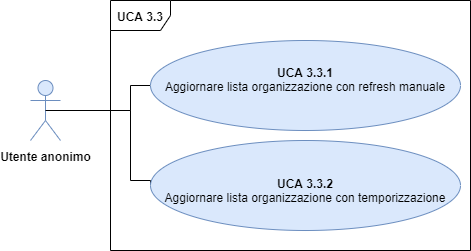
\includegraphics[scale=0.5, center]{Sezioni/UseCase/Immagini/UCA3.3.png}
	\caption{UCA 3.3 - Aggiornare lista \glo{organizzazioni}}
\end{figure}

\begin{itemize} 
	\item \textbf{Attori primari:} Utente anonimo, Utente riconosciuto
	\item \textbf{Precondizione:} L'utente è autenticato e può aggiornare la lista delle \glo{organizzazioni}.
	\item \textbf{Postcondizione:} L'utente ha aggiornato la lista di tutte le \glo{organizzazioni}.
	\item \textbf{Scenario principale:} L'utente ha la necessità di aggiornare la lista e può farlo manualmente con l'apposita funzionalità [UCA 3.3.1] o sarà fatto automaticamente dopo un determinato lasso di tempo [UCA 3.3.2].
	\item \textbf{Scenario alternativo 1:} Se il tentativo di scaricare la lista fallisce viene visualizzato all'utente un messaggio di errore che lo informa di tale problema [UCA 8.3.1].
	\item \textbf{Scenario alternativo 2:} Se non è presente nessuna lista delle \glo{organizzazioni} viene visualizzato all'utente un messaggio di errore che lo informa di tale problema [UCA 8.3.2];
	\item \textbf{Estensioni:}
	\begin{itemize}
		\item UCA 8.3.1 - Visualizzazione di un messaggio di errore che informa del tentativo fallito di scaricare la lista;
		\item UCA 8.3.2 - Visualizzazione di un messaggio di errore che informa che non è salvata nessuna lista delle \glo{organizzazioni}.
	\end{itemize}
\end{itemize}

\subsubsection{UCA 3.3.1 - Aggiornare lista organizzazione con refresh manuale}%fish level
\begin{itemize}
	\item \textbf{Attori primari:} Utente anonimo, Utente riconosciuto
	\item \textbf{Precondizione:} L'utente anonimo sceglie di eseguire la funzionalità aggiornamento della lista dell'\glo{organizzazione} attraverso la modalità di \glo{refresh manuale}.
	\item \textbf{Postcondizione:} La lista delle \glo{organizzazioni} è aggiornata.	
	\item \textbf{Scenario principale:} Aggiornamento della lista delle organizzazione con il refresh manuale.
	\item \textbf{Generalizzazione:}
	\begin{enumerate}
	\item UCA 3.3 - Aggiornare lista organizzazioni.
	\end{enumerate}
\end{itemize}

\subsubsection{UCA 3.3.2 - Aggiornare lista organizzazione con temporizzazione}%fish level
\begin{itemize} 
	\item \textbf{Attori primari:} Utente anonimo, Utente riconosciuto
	\item \textbf{Precondizione:} L'utente anonimo sceglie di eseguire la funzionalità aggiornamento della lista dell'\glo{organizzazione} attraverso la modalità \glo{temporizzazione}.
	\item \textbf{Postcondizione:} La lista delle \glo{organizzazioni} è aggiornata.
	\item \textbf{Scenario principale:} Aggiornamento della lista delle organizzazione con temporizzazione.
	\item \textbf{Generalizzazione:}
	\begin{enumerate}
	\item UCA 3.3 - Aggiornare lista organizzazioni.
	\end{enumerate}	
\end{itemize}

\subsubsection{UCA 3.4 - Visualizzazione lista delle organizzazioni}%sea level

\begin{figure}[h]
	\centering	
	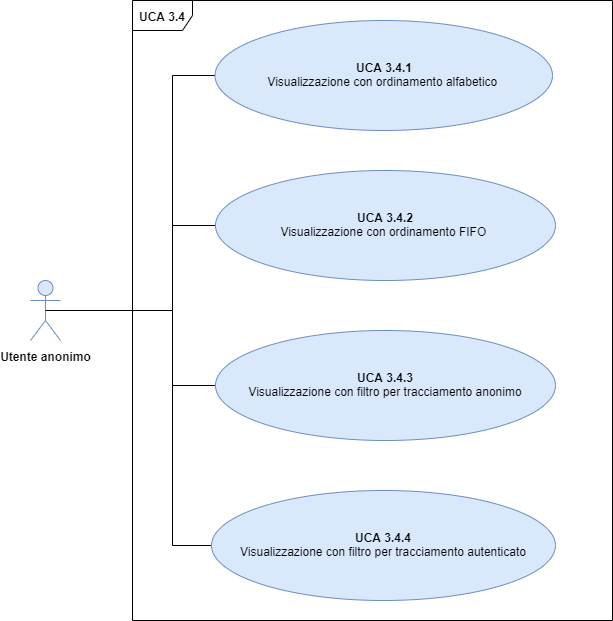
\includegraphics[scale=0.45, center]{Sezioni/UseCase/Immagini/UCA3.4.png}
	\caption{UCA 3.4 - Visualizzazione lista delle \glo{organizzazioni}}
\end{figure}

\begin{itemize} 
	\item \textbf{Attori primari:} Utente anonimo, Utente riconosciuto
	\item \textbf{Precondizione:}  L'utente è autenticato e può visualizzare la lista delle \glo{organizzazioni}.
	\item \textbf{Postcondizione:} L'utente visualizza la lista delle \glo{organizzazioni} nel modo che ritiene più opportuno.
	\item \textbf{Scenario principale:}	L'utente può scegliere come visualizzare la lista tramite diversi tipi di ordinamento:
	\begin{enumerate}
		\item Visualizzazione con ordinamento alfabetico [UCA 3.4.1];
		\item Visualizzazione con ordinamento \glo{FIFO} [UCA 3.4.2];
	\end{enumerate}
	\item \textbf{Scenario alternativo:} Se non è presente nessuna lista delle \glo{organizzazioni} viene visualizzato all'utente un messaggio di errore che lo informa di tale problema.
	\item \textbf{Estensioni:}
	\begin{itemize}
		\item UCA 8.3.2 - Visualizzazione di un messaggio di errore che informa che non è salvata nessuna lista delle organizzazioni.
	\end{itemize}
\end{itemize}

\subsubsection{UCA 3.4.1 - Visualizzazione con ordinamento alfabetico}%fish level
\begin{itemize}
	\item \textbf{Attori primari:} Utente anonimo, Utente riconosciuto
	\item \textbf{Precondizione:} L'utente autenticato può utilizzare la funzionalità di visualizzazione della lista secondo un ordinamento alfabetico (dalla a alla z) per il nome dell'\glo{organizzazione}.
	\item \textbf{Postcondizione:} Viene visualizzata la lista delle \glo{organizzazioni} in ordine alfabetico per il nome dell'\glo{organizzazione}.
	\item \textbf{Scenario principale:} Visualizzazione della lista delle organizzazioni con ordinamento alfabetico.
	\item \textbf{Generalizzazione:}
	\begin{enumerate}
	\item UCA 3.4 - Visualizzazione lista delle organizzazioni.
	\end{enumerate}	
\end{itemize}

\subsubsection{UCA 3.4.2 - Visualizzazione con ordinamento \glo{FIFO}}%fish level
\begin{itemize}	
	\item \textbf{Attori primari:} Utente anonimo, Utente riconosciuto
	\item \textbf{Precondizione:} L'utente autenticato può utilizzare la funzionalità di visualizzazione della lista secondo un ordinamento \glo{FIFO}.
	\item \textbf{Postcondizione:} Viene visualizzato la lista delle \glo{organizzazioni} secondo un ordinamento \glo{FIFO}.
	\item \textbf{Scenario principale:} Visualizzazione della lista delle organizzazioni con ordinamento \glo{FIFO}.
	\item \textbf{Generalizzazione:}
	\begin{enumerate}
	\item UCA 3.4 - Visualizzazione lista delle organizzazioni.
	\end{enumerate}	
\end{itemize}


\subsubsection{UCA 3.5 - Ricerca personalizzata delle organizzazioni}%sea level
\begin{figure}[h]
	\centering
	
	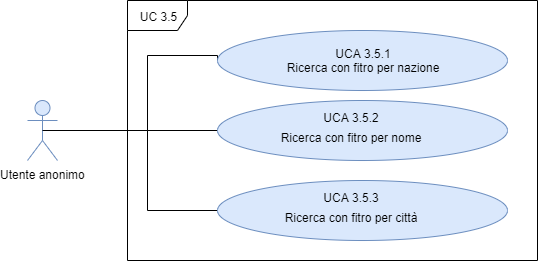
\includegraphics[scale=0.5, center]{Sezioni/UseCase/Immagini/UCA3.5.png}
	\caption{UCA 3.5 - Ricerca personalizzata delle \glo{organizzazioni}}
\end{figure}
\begin{itemize}
	\item \textbf{Attori primari:} Utente anonimo, Utente riconosciuto
	\item \textbf{Precondizione:} L'utente è autenticato e può svolgere ricerche riguardo le \glo{organizzazioni}.
	\item \textbf{Postcondizione:} Vengono forniti all'utente i risultati delle ricerche.
	\item \textbf{Scenario principale:} L'utente deve svolgere alcune ricerche e sceglie il metodo che più lo aggrada.
	\item \textbf{Flusso di eventi:} 
	\begin{enumerate}
		\item L'utente anonimo accede alla funzionalità di ricerca personalizzata della lista delle \glo{organizzazioni} per ricercare le \glo{organizzazioni} desiderate;
		\item L'utente ha la possibilità di effettuare la ricerca per nazione [UCA 3.5.1];
		\item L'utente ha la possibilità di effettuare la ricerca per nome [UCA 3.5.2];
		\item L'utente ha la possibilità di effettuare la ricerca per città [UCA 3.5.3].
	\end{enumerate}
	\item \textbf{Scenario alternativo:} Se non è presente nessuna lista delle \glo{organizzazioni} viene visualizzato all'utente un messaggio di errore che lo informa di tale problema [UCA 8.3.2].
	\item \textbf{Estensioni:}
	\begin{itemize}
		\item UCA 8.3.2 - Visualizzazione di un messaggio di errore che informa che non è salvata nessuna lista delle organizzazioni.
	\end{itemize}
\end{itemize}

\subsubsection{UCA 3.5.1 - Ricerca con filtro per nazione}%fish level
\begin{itemize}
	\item \textbf{Attori primari:} Utente anonimo, Utente riconosciuto
	\item \textbf{Precondizione:} L'utente autenticato può utilizzare la funzionalità di ricerca della lista per cercare le \glo{organizzazioni} di una certa nazione d'interesse.
	\item \textbf{Postcondizione:} Viene visualizzato la lista delle \glo{organizzazioni} che sono nella nazione scelta dall'utente.
	\item \textbf{Scenario principale:} Le ricerche vengono effettuate tramite un filtro per nazione.
	\item \textbf{Generalizzazione:}
	\begin{enumerate}
	\item UCA 3.5 - Ricerca personalizzata delle organizzazioni.
	\end{enumerate}	
\end{itemize}

\subsubsection{UCA 3.5.2 - Ricerca con filtro per nome}%fish level
\begin{itemize}
	\item \textbf{Attori primari:} Utente anonimo, Utente riconosciuto
	\item \textbf{Precondizione:} L'utente autenticato può utilizzare la funzionalità di ricerca della lista per cercare le \glo{organizzazioni} che hanno nel nome una sottostringa specificata dall'utente.
	\item \textbf{Postcondizione:} Viene visualizzato la lista delle \glo{organizzazioni} che hanno nel nome una sottostringa scelta dall'utente.
	\item \textbf{Scenario principale:} Le ricerche vengono effettuate tramite un filtro per nome.
	\item \textbf{Generalizzazione:}
	\begin{enumerate}
	\item UCA 3.5 - Ricerca personalizzata delle organizzazioni.
	\end{enumerate}	
\end{itemize}

\subsubsection{UCA 3.5.3 - Ricerca con filtro per città}%fish level
\begin{itemize}
	\item \textbf{Attori primari:} Utente anonimo, Utente riconosciuto
	\item \textbf{Precondizione:} L'utente autenticato può utilizzare la funzionalità di ricerca della lista per cercare le \glo{organizzazioni} di una certa città d'interesse.
	\item \textbf{Postcondizione:} Viene visualizzato la lista delle \glo{organizzazioni} che sono nella città scelta dall'utente.
	\item \textbf{Scenario principale:} Le ricerche vengono effettuate tramite un filtro per città.
	\item \textbf{Generalizzazione:}
	\begin{enumerate}
	\item UCA 3.5 - Ricerca personalizzata delle organizzazioni.
	\end{enumerate}	
\end{itemize}

\subsubsection{UCA 3.5.4 - Visualizzazione con filtro per tracciamento anonimo}%fish level
\begin{itemize}
	\item \textbf{Attori primari:} Utente anonimo, Utente riconosciuto
	\item \textbf{Precondizione:} L'utente autenticato può utilizzare la funzionalità di visualizzazione della lista che permettono un \glo{tracciamento anonimo}.
	\item \textbf{Postcondizione:} Viene visualizzato la lista delle \glo{organizzazioni} che richiedono il \glo{tracciamento anonimo}.
	\item \textbf{Scenario principale:} Visualizzazione della lista delle organizzazioni con filtro per tracciamento anonimo.
	\item \textbf{Generalizzazione:}
	\begin{enumerate}
	\item UCA 3.5 - Ricerca personalizzata delle organizzazioni.
	\end{enumerate}	
\end{itemize}

\subsubsection{UCA 3.5.5 - Visualizzazione con filtro per \glo{tracciamento autenticato}}%fish level
\begin{itemize}
	\item \textbf{Attori primari:} Utente anonimo, Utente riconosciuto
	\item \textbf{Precondizione:} L'utente autenticato può utilizzare la funzionalità di visualizzazione della lista che permette un \glo{tracciamento autenticato}.
	\item \textbf{Postcondizione:} Viene visualizzato la lista delle \glo{organizzazioni} che permettono il \glo{tracciamento autenticato}.
	\item \textbf{Scenario principale:} Visualizzazione della lista delle organizzazioni con filtro per \glo{tracciamento autenticato}.
	\item \textbf{Generalizzazione:}
	\begin{enumerate}
	\item UCA 3.5 - Ricerca personalizzata delle organizzazioni.
	\end{enumerate}	
\end{itemize}
%scritto da \PF{}
\subsubsection{UCA 4 - Inserimento modalità di tracciamento}%kite level

\begin{figure}[h]
	\centering	
	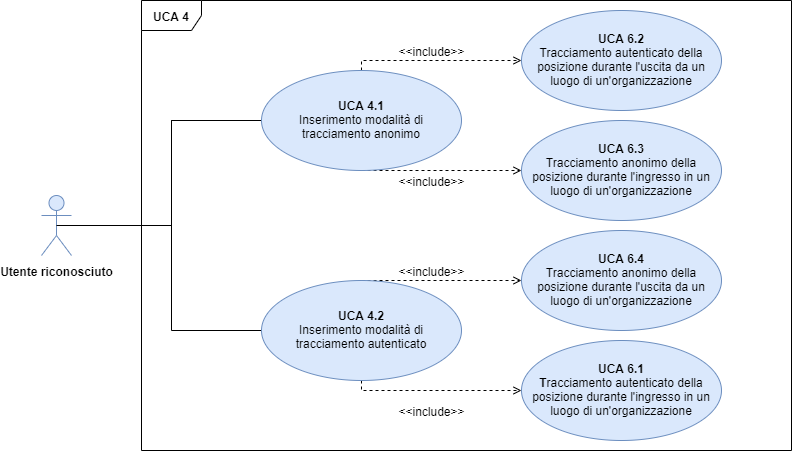
\includegraphics[scale=0.53, center]{Sezioni/UseCase/Immagini/UCA4.png}
	\caption{UCA 4 - Inserimento modalità di tracciamento}
\end{figure}

\begin{itemize}
	\item \textbf{Attori primari:} Utente riconosciuto
	\item \textbf{Precondizione:} L'utente si è autenticato con le credenziali LDAP\ap{G} nella organizzazione\ap{G} in cui si trova e vuole selezionare la modalità di tracciamento\ap{G}.
	\item \textbf{Postcondizione:} L'utente viene tracciato secondo la modalità da lui scelta precedentemente.
	\item \textbf{Scenario principale:} L'utente accede alla funzionalità di selezione della modalità di tracciamento\ap{G}.
	\item \textbf{Flusso di eventi:}
	\begin{enumerate}
		\item L'utente accede alla funzione di inserimento modalità di tracciamento;
		\item L'utente può scegliere la modalità di tracciamento anonimo\ap{G}\ap{G} [UCA 4.1] oppure la modalità di tracciamento\ap{G}autenticato\ap{G} [UCA 4.2].
	\end{enumerate}
\end{itemize}

\subsubsection{UCA 4.1 - Inserimento modalità di tracciamento anonimo}%sea level
\begin{itemize}
	\item \textbf{Attori primari:} Utente riconosciuto
	\item \textbf{Precondizione:} L'utente si è autenticato con le credenziali LDAP\ap{G} nella organizzazione\ap{G} in cui si trova e vuole selezionare la modalità di tracciamento anonimo\ap{G}\ap{G}].
	\item \textbf{Postcondizione:} L'utente viene tracciato secondo la modalità anonimo\ap{G}.
	\item \textbf{Scenario principale:} L'utente accede alla funzionalità inserimento modalità di tracciamento\ap{G} e inserisce la modalità anonimo\ap{G}.
	\item \textbf{Flusso di eventi:}
	\begin{enumerate}
	\item L'utente accede alla funzione di inserimento modalità di tracciamento anonimo\ap{G}\ap{G};
	\item L'utente inserisce la modalità di tracciamento anonimo\ap{G}\ap{G};
	\item Viene inviata al sistema l'uscita dell'utente autenticato dall'organizzazione\ap{G} [UCA 6.2];
	\item Viene inviato al sistema l'entrata dell'utente anonimo nell'organizzazione\ap{G} [UCA 6.3].
	\end{enumerate}
	\item \textbf{Inclusioni:}
	\begin{itemize}
		\item UCA 6.2 - Tracciamento\ap{G}autenticato della posizione durante l'uscita da un luogo di un'organizzazione\ap{G};
		\item UCA 6.3 - Tracciamento\ap{G}anonimo della posizione durante l'ingresso in un luogo di un'organizzazione\ap{G}.
	\end{itemize}
\end{itemize}

\subsubsection{UCA 4.2 - Inserimento modalità di tracciamento autenticato}%sea level
\begin{itemize}
	\item \textbf{Attori primari:} Utente riconosciuto
	\item \textbf{Precondizione:} L'utente si è autenticato con le credenziali LDAP\ap{G} nella organizzazione\ap{G} in cui si trova e vuole selezionare la modalità di tracciamento\ap{G}autenticato\ap{G}.
	\item \textbf{Postcondizione:} L'utente viene tracciato secondo la modalità autenticato\ap{G}.
	\item \textbf{Scenario principale:} L'utente accede alla funzionalità inserimento modalità di tracciamento\ap{G} e inserisce la modalità autenticato\ap{G}.
	\begin{enumerate}
		\item L'utente accede alla funzione di inserimento modalità di tracciamento\ap{G}autenticato\ap{G};
		\item L'utente inserisce la modalità di tracciamento\ap{G}autenticato\ap{G};
		\item Viene inviata al sistema l'uscita dell'utente anonimo dall'organizzazione\ap{G} [UCA 6.4];
		\item Viene inviato al sistema l'entrata dell'utente autenticato nell'organizzazione\ap{G} [UCA 6.1].
	\end{enumerate}
	\begin{itemize}
		\item UCA 6.4 - Tracciamento anonimo della posizione durante l'uscita da un luogo di un'organizzazione;
		\item UCA 6.1 - Tracciamento autenticato della posizione durante l'ingresso in un luogo di un'organizzazione.
	\end{itemize}
\end{itemize}

%\newpage


\subsubsection{UCA 5 - Visualizzazione dello storico accessi presso un'organizzazione}
\begin{figure}[h]
	\centering	
	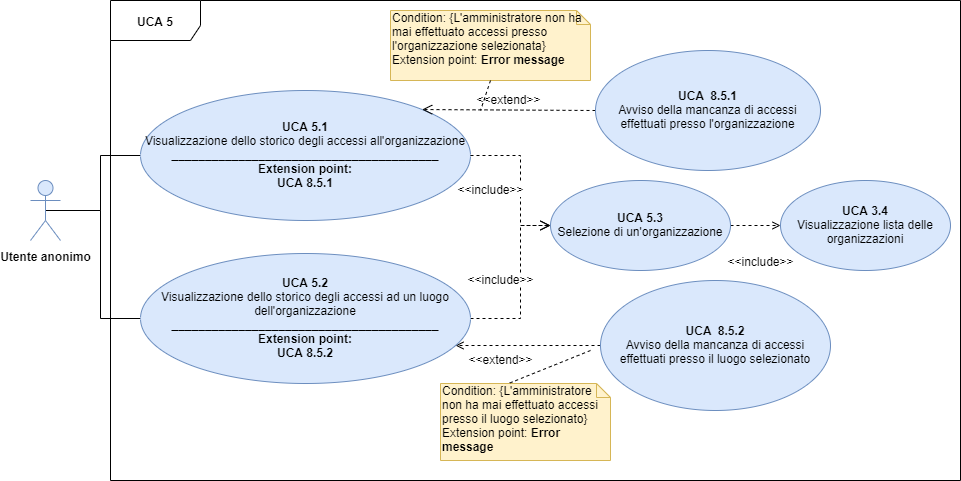
\includegraphics[scale=0.5]{sezioni/UseCase/Immagini/UCA5.png}
	\caption{UCA 5 - Visualizzazione dello storico accessi presso un'organizzazione}
\end{figure}

\begin{itemize}
    \item \textbf{Attori primari:} Utente Riconosciuto, Utente Anonimo.
    %\item \textbf{Attori secondari:}%opzionale
    \item \textbf{Precondizione:} L’utente ha precedentemente aggiunto l’organizzazione di cui vuole visualizzare i propri accessi alla lista delle organizzazione preferite.
    \item \textbf{Postcondizione:} L’utente visualizza nella schermata dell’applicazione la lista degli accessi effettuati presso i luoghi dell’organizzazione (con nome del luogo, timestamp di ingresso, di uscita, e tempo di permanenza).
    Se si trova all'interno di un luogo viene visualizzato il tempo passato al suo interno fino a quel momento.
    \item \textbf{Scenario principale:} L'utente può visualizzare la lista dei propri accessi presso un'organizzazione, se questa non è vuota, previa la selezione di un'organizzazione fra quelle presenti nella lista delle organizzazioni preferite dell'utente.
    %\item \textbf{Estensioni:}
    \item \textbf{Inclusioni:}
    \begin{itemize}
        \item UCA 5.1 - Visualizzazione della lista delle organizzazioni preferite;
        \item UCA 5.2 - Visualizzazione della lista degli accessi presso un'organizzazione.
    \end{itemize}
    \item \textbf{Estensioni:}
    \begin{enumerate}
        \item UCA 3.3.3 Visualizzazione di un messaggio di errore che informa che non è salvata nessuna lista delle organizzazioni.	
    \end{enumerate}	
\end{itemize}


\subsubsection{UCA 5.1 - Visualizzazione della lista delle organizzazioni preferite}
\begin{itemize}
    \item \textbf{Attori primari:} Utente Riconosciuto, Utente Anonimo.
    %\item \textbf{Attori secondari:}%opzionale
    \item \textbf{Precondizione:} L’utente ha precedentemente aggiunto le organizzazioni da visualizzare nella lista delle organizzazioni preferite.
    \item \textbf{Postcondizione:} L’utente visualizza nella schermata dell’applicazione la lista delle proprie organizzazioni preferite. 
    \item \textbf{Scenario principale:} L'utente può visualizzare la lista delle proprie organizzazioni preferite, se questa non è vuota, e da qui procedere con UCA 5.2.
    \item \textbf{Scenario alternativo:} L'utente non ha organizzazioni preferite, per cui viene visualizzato un avviso come indicato in UCA 5.1.1.
    \item \textbf{Flusso di eventi:}
    \begin{enumerate}
        \item L'utente seleziona la funzionalità "Storico accessi".
    \end{enumerate}
    \item \textbf{Estensioni:}
    \begin{itemize}
        \item UCA 5.1.1 - Avviso di assenza di organizzazioni preferite;
    \end{itemize}
    %\item \textbf{Inclusioni:}
\end{itemize}

\subsubsection{UCA 5.1.1 - Avviso di assenza di organizzazioni preferite}
\begin{itemize}
    \item \textbf{Attori primari:} Utente Riconosciuto, Utente Anonimo
    %\item \textbf{Attori secondari:}%opzionale
    \item \textbf{Precondizione:} l'utente non ha aggiunto alcuna organizzazione come preferita.
    \item \textbf{Postcondizione:} l'utente visualizza nella schermata un messaggio che lo avvisa della mancanza di organizzazioni.
\end{itemize}

\subsubsection{UCA 5.2 - Visualizzazione della lista degli accessi presso un'organizzazione}
\begin{itemize}
    \item \textbf{Attori primari:} Utente Riconosciuto, Utente Anonimo.
    %\item \textbf{Attori secondari:}%opzionale
    \item \textbf{Precondizione:} L'utente ha selezionato dalla lista delle organizzazioni preferite un'organizzazione di cui visualizzare i propri accessi.
    \item \textbf{Postcondizione:} L’utente visualizza nella schermata dell’applicazione la lista degli accessi effettuati presso i luoghi dell’organizzazione (con descrizione del luogo, timestamp di ingresso, di uscita, e tempo di permanenza).
    Se si trova all'interno di un luogo viene visualizzato il tempo passato al suo interno fino a quel momento.
    \item \textbf{Scenario principale:} L'utente può visualizzare tutti gli accessi da lui fatti presso i luoghi dell'organizzazione, in modalità di tracciamento anonimo e autenticato.
    \item \textbf{Scenario alternativo:} L'utente ha effettuato l'accesso presso il luogo dell'organizzazione ma non ne è ancora uscito. In questo caso, viene visualizzato un timer con il tempo trascorso dal momento in cui è entrato.
    Una volta uscito dal luogo, vale il comportamento descritto nello scenario principale. 
    \item \textbf{Flusso di eventi:}
    \begin{enumerate}
        \item L'utente esegue UCA 5.1;
        \item L'utente, per precondizione, ha selezionato un'organizzazione di cui visualizzare i propri accessi nei suoi luoghi.
    \end{enumerate}
    \item \textbf{Inclusioni:} % non sono sicuro sia corretto
    \begin{itemize}
        \item UCA 5.1 - Visualizzazione della lista delle organizzazioni preferite.
    \end{itemize}
    \item \textbf{Estensioni:}
    \begin{itemize}
        \item UCA 5.2.1 - Avviso di assenza di accessi presso i luoghi di un’organizzazione.
    \end{itemize}
    %\item \textbf{Inclusioni:}
\end{itemize}

\subsubsection{UCA 5.2.1 - Avviso di assenza di accessi presso i luoghi di un’organizzazione}
\begin{itemize}
    \item \textbf{Attori primari:} Utente Riconosciuto, Utente Anonimo.
    %\item \textbf{Attori secondari:}%opzionale
    \item \textbf{Precondizione:} L'utente ha selezionato dalla lista delle organizzazioni preferite un'organizzazione di cui visualizzare i propri accessi, ma non ha mai effettuato accesso ai luoghi dell'organizzazione.
    \item \textbf{Postcondizione:} L'utente visualizza nella schermata un messaggio che lo avvisa della mancanza di accessi nei luoghi dell'organizzazione.
\end{itemize}

% \begin{figure}[h]
% 	\centering
% 	\caption{UCA 6.1 - Ordinamento della lista degli accessi presso un’organizzazione}
% 	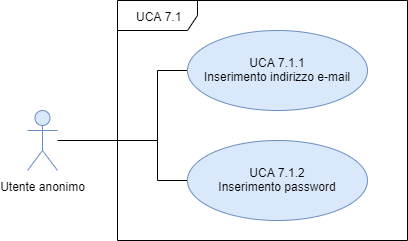
\includegraphics[scale=0.5]{sezioni/UseCase/Immagini/UCA7.1.png}
% \end{figure}
\subsubsection{UCA 5.2.2 - Ordinamento per data (decrescente) della lista degli accessi}
\begin{itemize}
    \item \textbf{Attori primari:} Utente Riconosciuto, Utente Anonimo.
    %\item \textbf{Attori secondari:}%opzionale
    \item \textbf{Precondizione:} L’utente ha a disposizione una lista di accessi presso uno o più luoghi di un organizzazione preferita.
    \item \textbf{Postcondizione:} L’utente ottiene la lista di accessi iniziale riordinata in ordine decrescente (ovvero una data più recente è considerata più grande di una data meno recente).
    \item \textbf{Inclusioni:} % non sono sicuro sia corretto
    \begin{itemize}
        \item UCA 5.2 - Visualizzazione della lista degli accessi presso un'organizzazione.
    \end{itemize}
    \item \textbf{Flusso di eventi:}
    \begin{enumerate}
        \item L'utente esegue il caso d'uso UCA 5.2
        \item L'utente seleziona la funzionalità "Ordinamento lista accessi".
        \item L'utente sceglie la funzionalità "Ordinamento per data (decrescente)".
    \end{enumerate}
\end{itemize}

\subsubsection{UCA 5.2.3 - Ordinamento per data (crescente) della lista degli accessi}
\begin{itemize}
    \item \textbf{Attori primari:} Utente Riconosciuto, Utente Anonimo.
    %\item \textbf{Attori secondari:}%opzionale
    \item \textbf{Precondizione:} l’utente ha a disposizione una lista di accessi presso uno o più luoghi di un organizzazione preferita.
    \item \textbf{Postcondizione:} l’utente ottiene la lista di accessi iniziale riordinata in ordine crescente (ovvero una data meno recente è considerata più piccola di una data più recente).
    \item \textbf{Inclusioni:} % non sono sicuro sia corretto
    \begin{itemize}
        \item UCA 5.2 - Visualizzazione della lista degli accessi presso un'organizzazione.
    \end{itemize}
    \item \textbf{Flusso di eventi:}
    \begin{enumerate}
        \item L'utente esegue il caso d'uso UCA 5.2
        \item l'utente seleziona la funzionalità "Ordinamento lista accessi".
        \item l'utente sceglie la funzionalità "Ordinamento per data (crescente)".
    \end{enumerate}
\end{itemize}

\subsubsection{UCA 5.2.4 - Filtro per luogo della lista degli accessi presso un’organizzazione}
\begin{itemize}
    \item \textbf{Attori primari:} Utente Riconosciuto, Utente Anonimo.
    \item \textbf{Precondizione:} l’utente ha a disposizione una lista di accessi presso uno o più luoghi di un organizzazione preferita.
    \item \textbf{Precondizione:} l’utente ottiene la lista di accessi iniziale presso un singolo luogo selezionato (che può coincidere con la lista di partenza se l’organizzazione ha un singolo luogo a disposizione oppure essere vuota).
    \item \textbf{Inclusioni:} % non sono sicuro sia corretto
    \begin{itemize}
        \item UCA 5.2 - Visualizzazione della lista degli accessi presso un'organizzazione.
    \end{itemize}
    \item \textbf{Flusso di eventi:}
    \begin{enumerate}
        \item L'utente esegue il caso d'uso UCA 5.2
        \item l’utente seleziona la funzionalità “Filtro per luogo”.
        \item l’utente seleziona un luogo dell’organizzazione di cui mostrare gli accessi.
    \end{enumerate}
\end{itemize}
%\newpage

\subsubsection{UCA 6 - Tracciamento posizione}%kite level

\begin{figure}[h]
	\centering
	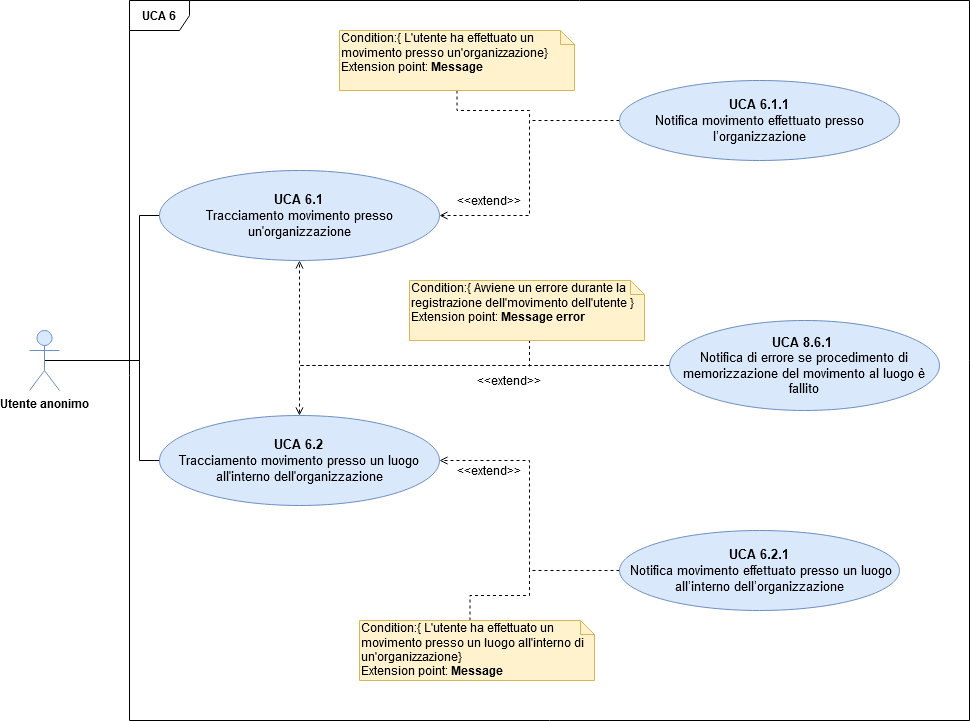
\includegraphics[scale=0.3]{sezioni/UseCase/Immagini/UCA6.png}
	\caption{Tracciamento\ap{G} posizione}
\end{figure}

\begin{itemize}
	\item \textbf{Attori primari:} Utente anonimo, Utente riconosciuto
	\item \textbf{Attori secondari:} Servizi/o di localizzazione (GPS\ap{G}, rete cellulare)
	\item \textbf{Precondizione:} L'utente autenticato\ap{G} con credenziali Stalker sta per entrare o sta per uscire da un luogo dell'organizzazione che richiede il tracciamento;ì.
	\item \textbf{Postcondizione:} Viene memorizzato dal sistema il timestamp\ap{G} i momenti in cui è avvenuto il tracciamento\ap{G}, dove è avvenuto e il tempo trascorso al suo interno.
	\item \textbf{Scenario principale:} L'utente si trova nei pressi o sta per uscire da un luogo dell'organizzazione che richiede il tracciamento\ap{G}. Viene salvato il timestamp\ap{G} di entrata ed uscita dall'organizzazione e viene salvato il tempo trascorso all'interno dell'organizzazione.
\end{itemize}

\subsubsection{UCA 6.1 - Tracciamento autenticato della posizione durante l'ingresso in un luogo di un'organizzazione}
\begin{itemize}
	\item \textbf{Attori primari:} Utente riconosciuto
	\item \textbf{Attori secondari:} Servizi/o di localizzazione (GPS\ap{G}, rete cellulare), server LDAP\ap{G} dell'organizzazione
	\item \textbf{Precondizione:} L'utente sta per entrare (ovvero si trova nei pressi) in un luogo dell'organizzazione che richiede il tracciamento\ap{G}.
	\item \textbf{Postcondizione:} Viene registrato l'ingresso nel luogo dell'organizzazione in una certa data e ora (timestamp\ap{G}).
	\item \textbf{Scenario principale:} L'utente, tramite i/il servizio/i di localizzazione, verifica il momento in cui entra al suo interno. Una volta entrato al suo interno, verifica di potersi autenticare correttamente con le credenziali dell'organizzazione [UCA 6.1.2]: se riesce, memorizza nel sistema la data e ora di ingresso nel luogo [UCA 6.1.1]. Infine, viene informato l'utente dell'ingresso riuscito.
	\item \textbf{Scenario alternativo:} Il tentativo di autenticazione\ap{G} presso l'organizzazione o l'invio delle credenziali fallisce. Viene informato l'utente.
	\item \textbf{Estensioni:}
	\begin{enumerate}
		\item UCA 6.1.3;
		\item UCA 6.1.4.
	\end{enumerate}
	\item \textbf{Inclusioni:}
	\begin{enumerate}
		\item UCA 6.1.1;
		\item UCA 6.1.2.
	\end{enumerate}
\end{itemize}

% DA 6.1.1 A 6.1.4 RICHIEDONO UN CAMBIO DI NUMERAZIONE PERCHE' NON SONO SOLO RELATIVI A UCA 6.1
\subsubsection{UCA 6.1.1 - Invio timestamp relativo all'ingresso/uscita in/da un luogo}
\begin{itemize}
	\item \textbf{Attori primari:} Utente riconosciuto, Utente anonimo
	\item \textbf{Precondizione:} L'utente ha verificato di trovarsi nei pressi di un luogo che richiede il tracciamento\ap{G} autenticato\ap{G}.
	\item \textbf{Postcondizione:} Viene registrato il timestamp\ap{G} relativo all'ingresso dell'utente nel luogo dell'organizzazione.
\end{itemize}

\subsubsection{UCA 6.1.2 - Verifica correttezza delle credenziali di accesso all'organizzazione}
\begin{itemize}
	\item \textbf{Attori primari:} Utente riconosciuto
	\item \textbf{Attori secondari:} Server\ap{G} dell'organizzazione
	\item \textbf{Precondizione:} L'utente, in quanto riconosciuto, possiede credenziali per autenticarsi presso l'organizzazione;
	\item \textbf{Postcondizione:} Viene verificata o meno la validità delle credenziali fornite: esse sono valide se la verifica va a buon fine.
\end{itemize}

\subsubsection{UCA 6.1.3 - Notifica di errore se procedimento di memorizzazione dell'accesso al luogo è fallito}
\begin{itemize}
	\item \textbf{Attori primari:} Utente riconosciuto, Utente anonimo
	\item \textbf{Precondizione:} Avviene un errore durante la registrazione dell'accesso dell'utente.
	\item \textbf{Postcondizione:} Viene notificato l'errore all'utente.
\end{itemize}

\subsubsection{UCA 6.1.4 - Notifica di avvenuta memorizzazione dei dati dell'accesso}
\begin{itemize}
	\item \textbf{Attori primari:} Utente riconosciuto, Utente anonimo
	\item \textbf{Precondizione:} Il processo di memorizzazione dei dati dell'accesso nel sistema è avvenuto correttamente.
	\item \textbf{Postcondizione:} Viene notificato l'utente dell'avvenuto salvataggio.
\end{itemize}

\subsubsection{UCA 6.2 - Tracciamento riconosciuto della posizione durante l'uscita in un luogo di un'organizzazione}
\begin{itemize}
	\item \textbf{Attori primari:} Utente riconosciuto
	\item \textbf{Attori secondari:} Servizi/o di localizzazione (GPS\ap{G}, rete cellulare), server LDAP\ap{G} dell'organizzazione
	\item \textbf{Precondizione:} L'utente sta per uscire da un luogo dell'organizzazione che richiede il tracciamento\ap{G}.
	\item \textbf{Postcondizione:} Viene registrato l'uscita dal luogo dell'organizzazione in una certa data e ora (timestamp\ap{G}).
	\item \textbf{Scenario principale:} L'utente, quando verifica tramite i/il servizi/o di localizzazione che sta per uscire da un luogo dell'organizzazione, verifica il momento in cui avviene l'uscita. Quando esce, verifica di potersi autenticare correttamente con le credenziali dell'organizzazione [UCA 6.1.2]: se riesce, memorizza nel sistema la data e ora di uscita dal luogo [UCA 6.1.1]. Infine, viene informato l'utente dell'uscita riuscita. La combinazione di ingresso effettuato in precedenza e dell'uscita effettuata formano un accesso, ora ritrovabile in Storico accessi [UCA 5].
	\item \textbf{Scenario alternativo:} Il tentativo di autenticazione\ap{G} presso l'organizzazione o l'invio delle credenziali fallisce. Viene informato l'utente.
	\item \textbf{Estensioni:}
	\begin{enumerate}
		\item UCA 6.1.3;
		\item UCA 6.1.4.
	\end{enumerate}
	\item \textbf{Inclusioni:}
	\begin{enumerate}
		\item UCA 6.1.1;
		\item UCA 6.1.2.
	\end{enumerate}
\end{itemize}

\subsubsection{UCA 6.3 - Tracciamento anonimo della posizione durante l'ingresso in un luogo di un'organizzazione}
\begin{itemize}
	\item \textbf{Attori primari:} Utente anonimo
	\item \textbf{Attori secondari:} Servizi/o di localizzazione (GPS\ap{G}, rete cellulare)
	\item \textbf{Precondizione:} L'utente sta per entrare (ovvero si trova nei pressi) in un luogo dell'organizzazione che richiede il tracciamento\ap{G}.
	\item \textbf{Postcondizione:} Viene registrato l'ingresso nel luogo dell'organizzazione in una certa data e ora (timestamp\ap{G}).
	\item \textbf{Scenario principale:} L'utente, tramite i/il servizio/i di localizzazione, verifica il momento in cui entra al suo interno. Quando entra al suo interno memorizza nel sistema la data e ora di ingresso nel luogo [UCA 6.1.1]. Infine, viene informato l'utente dell'ingresso riuscito.
	\item \textbf{Scenario alternativo:} Il tentativo di invio delle credenziali fallisce. Viene informato l'utente.
	\item \textbf{Estensioni:}
	\begin{enumerate}
		\item UCA 6.1.3;
		\item UCA 6.1.4.
	\end{enumerate}
	\item \textbf{Inclusioni:}
	\begin{enumerate}
		\item UCA 6.1.1.
	\end{enumerate}
\end{itemize}

\subsubsection{UCA 6.4 - Tracciamento anonimo della posizione durante l'uscita in un luogo di un'organizzazione}
\begin{itemize}
	\item \textbf{Attori primari:} Utente anonimo
	\item \textbf{Attori secondari:} Servizi/o di localizzazione (GPS\ap{G}, rete cellulare)
	\item \textbf{Precondizione:} L'utente sta per uscire da un luogo dell'organizzazione che richiede il tracciamento\ap{G}.
	\item \textbf{Postcondizione:} Viene registrato l'uscita dal luogo dell'organizzazione in una certa data e ora (timestamp\ap{G}).
	\item \textbf{Scenario principale:} L'utente, quando verifica tramite i/il servizi/o di localizzazione che sta per uscire da un luogo dell'organizzazione, verifica il momento in cui avviene l'uscita. Quando esce, memorizza nel sistema la data e ora di uscita dal luogo [UCA 6.1.1]. Infine, viene informato l'utente dell'uscita riuscita. La combinazione di ingresso effettuato in precedenza e dell'uscita effettuata formano un accesso, ora ritrovabile in Storico accessi [UCA 5].
	\item \textbf{Scenario alternativo:} Il tentativo di invio delle credenziali fallisce. Viene informato l'utente.
	\item \textbf{Estensioni:}
	\begin{enumerate}
		\item UCA 6.1.3;
		\item UCA 6.1.4.
	\end{enumerate}
	\item \textbf{Inclusioni:}
	\begin{enumerate}
		\item UCA 6.1.1.
	\end{enumerate}
\end{itemize}
\subsubsection{UCA 7 - Autenticazione con credenziali LDAP}%kite level

\begin{figure}[h]
	\centering
	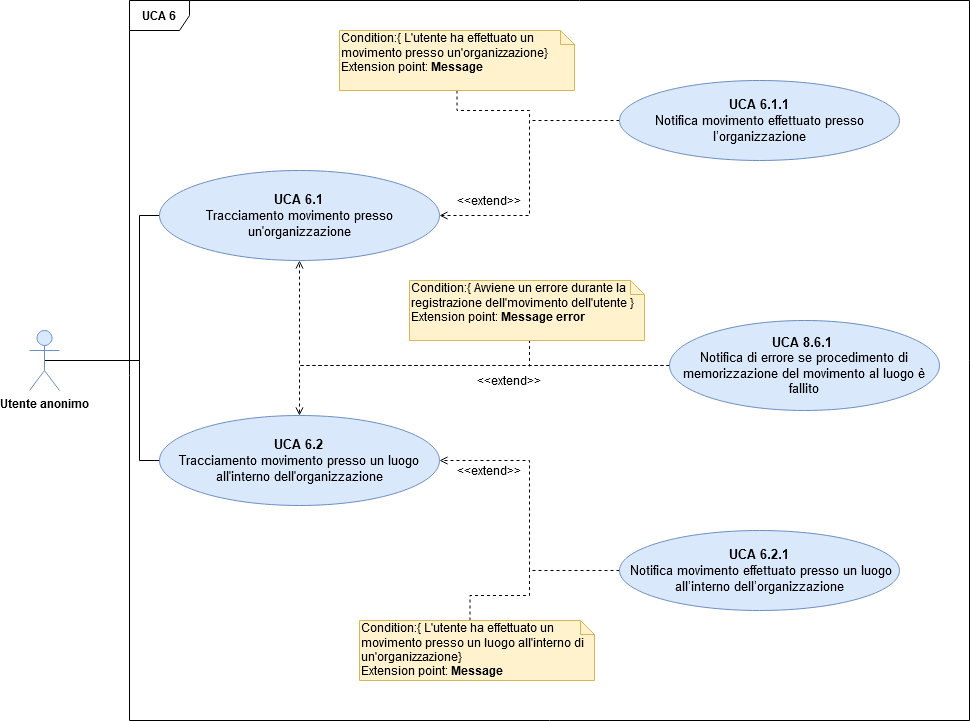
\includegraphics[scale=0.3]{sezioni/UseCase/Immagini/UCA6.png}
	\caption{Tracciamento\ap{G} posizione in un luogo di un'organizzazione\ap{G}}
\end{figure}

\begin{itemize}
	\item \textbf{Attori primari:} Utente anonimo 
	\item \textbf{Attori secondari:} server LDAP\ap{G} dell'organizzazione.
	\item \textbf{Precondizione:} L'utente autenticato con credenziali Stalker sta per effettuare l'autenticazione con credenziali LDAP.
	\item \textbf{Postcondizione:} L'utente è autenticato all'interno dell'organizzazione\ap{G} con credenziali LDAP.
	\item \textbf{Scenario principale:} L'utente autenticato come utente anonimo effettua l'autenticazione con credenziali LDAP\ap{G} [UCA 7.1] per autenticarsi come utente riconosciuto.
\end{itemize}

\subsubsection{UCA 7.1 - Inserimento credenziali}
\begin{itemize}
	\item \textbf{Attori primari:} Utente anonimo 
	\item \textbf{Attori secondari:} server LDAP\ap{G} dell'organizzazione.
	\item \textbf{Precondizione:} L'utente autenticato con credenziali Stalker inserisce le proprie credenziali LDAP/ap{G}.
	\item \textbf{Postcondizione:} L'utente ha inserito le proprie credenziali LDAP\ap{G}.
	\item \textbf{Scenario principale:}: L'utente inserisce le proprie credenziali LDAP\ap{G} per potersi autenticare.
	\item \textbf{Flusso di eventi:}
	\begin{enumerate}
		\item L'utente inserisci l'indirizzo e-mail [UCA 7.1.1];
		\item L'utente inserisce la password [UCA 7.1.2].
	\end{enumerate}
	\item \textbf{Scenario alternativo:} Il tentativo di autenticazione\ap{G} fallisce perché le credenziali inserite sono errate.
	\item \textbf{Estensioni:}
	\begin{enumerate}
		\item UCA 8.1.7 - Visualizzazione messaggio di errore credenziali errate.
	\end{enumerate}
\end{itemize}

\subsubsection{UCA 7.1.1 - Inserimento indirizzo e-mail}%fish level
\begin{itemize}
	\item \textbf{Attori primari:} Utente anonimo
	\item \textbf{Precondizione:} L'utente inserisce il proprio l'indirizzo e-mail.
	\item \textbf{Postcondizione:} L'utente ha inserito il proprio indirizzo e-mail.
\end{itemize}

\subsubsection{UCA 7.1.2 - Inserimento password}%fish level
\begin{itemize}
	\item \textbf{Attori primari:} Utente anonimo
	\item \textbf{Precondizione:} L'utente inserisci il proprio la password
	\item \textbf{Postcondizione:} L'utente ha inserito la propria password.
\end{itemize}

%scritto da \PF{}
\subsubsection{UCA 8.1.1 - Visualizzazione messaggio di errore in caso di account con l'e-mail inserita già presente}%fish level
\begin{itemize}
\item \textbf{Attori primari:} Utente non autenticato
%\item \textbf{Attori secondari:}%opzionale
\item \textbf{Precondizione:} L'utente non è registrato e ha inserito nel campo indirizzo e-mail un valore già presente nel sistema.
\item \textbf{Postcondizione:} L'indirizzo e-mail inserito dall'utente è già presente nel sistema, pertanto riceve un messaggio di errore esplicativo che lo esorta a scegliere una nuova password.
\end{itemize}

\subsubsection{UCA 8.1.2 - Visualizzazione messaggio di errore in caso di password troppo debole}%fish level
\begin{itemize}
\item \textbf{Attori primari:} Utente non autenticato
%\item \textbf{Attori secondari:}%opzionale
\item \textbf{Precondizione:} L'utente non è registrato e ha inserito una password poco sicura.
\item \textbf{Postcondizione:} La password inserita dall'utente risulta essere poco sicura per il sistema, pertanto riceve un messaggio di errore che gli intima di sceglierne una più sicura.
\end{itemize}

\subsubsection{UCA 8.1.3 - Visualizzazione messaggio di errore in caso di password e conferma password diverse}%fish level
\begin{itemize}
\item \textbf{Attori primari:} Utente non autenticato
%\item \textbf{Attori secondari:}%opzionale
\item \textbf{Precondizione:} L'utente non è registrato e ha inserito nei campi relativi alla password e conferma password valori differenti.
\item \textbf{Postcondizione:} La password inserita dall'utente è diversa da quella inserita nel campo conferma password, pertanto riceve un messaggio di errore esplicativo.
\end{itemize}

\subsubsection{UCA 8.1.4 - Visualizzazione messaggio di errore credenziali errate}%fish level
\begin{itemize}
    \item \textbf{Attori primari:} Utente non autenticato
    \item \textbf{Precondizione:}  L'utente non è autenticato.
    \item \textbf{Postcondizione:} L'utente visualizza un messaggio di errore a causa delle credenziali inserite in modo errato.
\end{itemize}

\subsubsection{UCA 8.3.1 - Visualizzazione di un messaggio di errore che informa del tentativo fallito di scaricare la lista}%fish level
\begin{itemize}
\item \textbf{Attori primari:} Utente anonimo
\item \textbf{Precondizione:} L'utente esegue l'azione di scaricare la lista delle \glo{organizzazioni} ma fallisce.
\item \textbf{Postcondizione:} Viene visualizzato un messaggio d'errore che informa che il tentativo di scaricare la lista è fallito.

\end{itemize}

\subsubsection{UCA 8.3.2 - Visualizzazione di un messaggio di errore che informa che non è salvata nessuna lista delle organizzazioni}%fish level
\begin{itemize}
	\item \textbf{Attori primari:} Utente anonimo
	\item \textbf{Precondizione:} La lista delle \glo{organizzazioni} non è presente nel dispositivo dell'utente.
	\item \textbf{Postcondizione:} Viene visualizzato un messaggio di errore che informa che nel dispositivo non è presente la lista delle \glo{organizzazioni}.
\end{itemize}

\subsubsection{UCA 8.5.1 - Avviso della mancanza di accessi effettuati presso l'organizzazione selezionata}
\begin{itemize}
    \item \textbf{Attori primari:} Utente anonimo
    \item \textbf{Precondizione:} L'utente ha tentato di visualizzare lo \glo{storico degli accessi} di un'\glo{organizzazione} nella quale non è mai entrato.
    \item \textbf{Postcondizione:} Viene mostrato un messaggio che avvisa l'utente della mancanza di accessi presso l'\glo{organizzazione} selezionata.
\end{itemize}

\subsubsection{UCA 8.5.2 - Avviso della mancanza di accessi effettuati presso il luogo selezionato}
\begin{itemize}
    \item \textbf{Attori primari:} Utente anonimo
    \item \textbf{Precondizione:} L'utente ha tentato visualizzare lo \glo{storico degli accessi} di un luogo di un'\glo{organizzazione} nella quale non è mai entrato.
    \item \textbf{Postcondizione:} L'utente visualizza un messaggio che lo avvisa della mancanza di accessi nel luogo scelto.
\end{itemize}

\subsubsection{UCA 8.6.1 - Notifica di errore se procedimento di memorizzazione del movimento al luogo è fallito}
\begin{itemize}
	\item \textbf{Attori primari:} Utente riconosciuto, Utente anonimo
	\item \textbf{Precondizione:} Avviene un errore durante la registrazione dell'accesso dell'utente.
	\item \textbf{Postcondizione:} Viene notificato l'errore all'utente.
\end{itemize}

\subsubsection{UCA 8.7.1 - Visualizzazione messaggio di errore credenziali LDAP aziendali errate}
\begin{itemize}
	\item \textbf{Attori primari:} Utente anonimo
	\item \textbf{Precondizione:} L'utente ha inserito delle credenziali LDAP non riconosciute dal server aziendale.
	\item \textbf{Postcondizione:} Viene notificato l'errore all'utente.
\end{itemize}
\subsubsection{UCS 1 - Accesso al server}%kite level

\begin{itemize}
\item \textbf{Attori primari:} Amministratore non autenticato
\item \textbf{Precondizione:} L'amministratore non è autenticato.
\item \textbf{Postcondizione:} L'amministratore viene autenticato all'interno del sistema tramite \glo{autenticazione}.
\item \textbf{Scenario principale:} L'amministratore non autenticato può accedere, tramite l'\glo{autenticazione} [UCS 1.1], al server. 
%\item \textbf{Estensioni:}
\end{itemize}

\subsubsection{UCS 1.1 - Autenticazione al Server}

\begin{figure}[h]
    \centering
    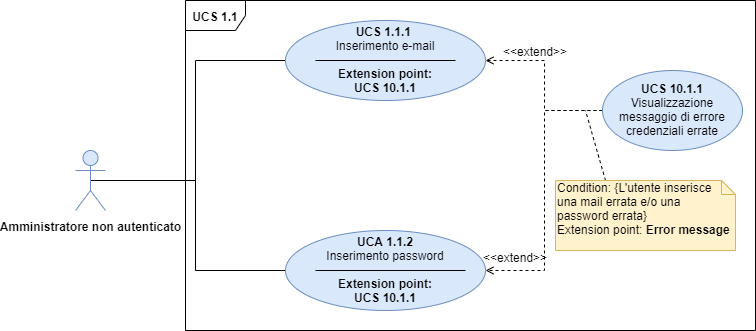
\includegraphics[scale=0.6]{Sezioni/UseCase/Immagini/UCS1.1.png}
    \caption{UCS 1.1 - \glo{Autenticazione} al Server}
\end{figure}

\begin{itemize}
\item \textbf{Attori primari:} Amministratore non autenticato
\item \textbf{Precondizione:} L'amministratore non è autenticato.
\item \textbf{Postcondizione:} L'amministratore è stato autenticato e può avere accesso alle funzionalità offerte dal sistema.
\item \textbf{Scenario principale:} Amministratore non identificato inserisce e-mail e la password per autenticarsi al server.
\item \textbf{Scenario alternativo 1:} L'amministratore tenta di accede con delle credenziali errate [UCS 10.1.1].
\item \textbf{Scenario alternativo 2:} Qualora l'amministratore non dovesse ricordarsi la password può selezionare la funzionalità "password dimenticata" per reimpostarla [UCS 1.3].
\item \textbf{Flusso di eventi:}
    \begin{enumerate}
        \item Inserimento e-mail [UCS 1.1.1];
        \item Inserimento password [UCS 1.1.2];
        \item L'amministratore seleziona la funzionalità di accesso.
    \end{enumerate}
    \item \textbf{Inclusioni:}
	\begin{itemize}		
		\item UCS 1.1.1 - Inserimento e-mail;
		\item UCS 1.1.2 - Inserimento password.
	\end{itemize}
    \item \textbf{Estensioni:}
    \begin{itemize}
		\item UCS 10.1.1 - Visualizzazione messaggio di errore credenziali errate;
		\item UCS 1.3 - Password dimenticata.
	\end{itemize}
\end{itemize}

\subsubsection{UCS 1.1.1 - Inserimento e-mail}%sea level
\begin{itemize}
\item \textbf{Attori primari:} Amministratore non autenticato
%\item \textbf{Attori secondari:}%opzionale
\item \textbf{Precondizione:} L'amministratore non è autenticato.
\item \textbf{Postcondizione:} L'amministratore ha inserito la propria e-mail.
\item \textbf{Scenario principale:} Inserimento dell'e-mail per l'autenticazione al Server.
\end{itemize}

\subsubsection{UCS 1.1.2 - Inserimento password}%sea level
\begin{itemize}
\item \textbf{Attori primari:} Amministratore non autenticato
%\item \textbf{Attori secondari:}%opzionale
\item \textbf{Precondizione:} L'amministratore non è autenticato.
\item \textbf{Postcondizione:} L'amministratore ha inserito la propria password.
\item \textbf{Scenario principale:} Inserimento della password per l'autenticazione al Server.
\end{itemize}



\subsubsection{UCS 1.3 - Password dimenticata}%sea level

\begin{figure}[h]
	\centering
	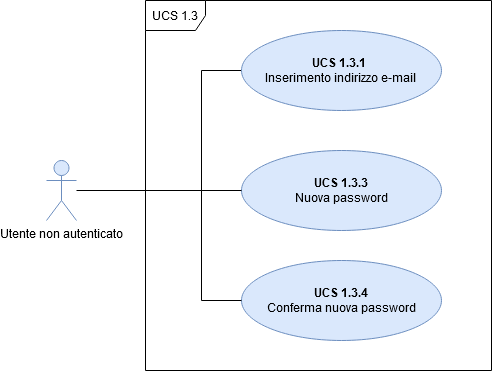
\includegraphics[scale=0.6]{Sezioni/UseCase/Immagini/UCS1.3.png}
	\caption{UCS 1.3 - Password dimenticata}
\end{figure}

\begin{itemize}
\item \textbf{Attori primari:} Amministratore non autenticato
%\item \textbf{Attori secondari:}%opzionale
\item \textbf{Precondizione:}  L'amministratore non è autenticato.
\item \textbf{Postcondizione:} L'amministratore ha cambiato password con successo, la quale è stata salvata presso il sistema.
\item \textbf{Scenario principale:} L'amministratore non autenticato inserisce i dati necessari per cambiare la propria password.
\item \textbf{Flusso di eventi:}
    \begin{enumerate}
        \item Inserimento e-mail [UCS 1.3.1];
        \item E-mail cambio password [UCS 1.3.2];
        \item Nuova password [UCS 1.3.3];
        \item Conferma nuova password [UCS 1.3.4];
    \end{enumerate}
\end{itemize}

\subsubsection{UCS 1.3.1 - Inserimento e-mail}
\begin{itemize}
\item \textbf{Attori primari:} Amministratore non autenticato
\item \textbf{Precondizione:} L'amministratore non è autenticato. %è nella schermata di password dimenticata
\item \textbf{Postcondizione:} L'amministratore ha inserito l'e-mail.
\item \textbf{Scenario principale:} Inserimento dell'e-mail per cambiare la password.
\end{itemize}

\subsubsection{UCS 1.3.2 - E-mail cambio password}
\begin{itemize}
\item \textbf{Attori primari:} Amministratore non autenticato
\item \textbf{Precondizione:} L'amministratore non è autenticato.
\item \textbf{Postcondizione:} L'amministratore riceve l'email per il cambio password, ne consegue la necessità di reimpostare la password.
\item \textbf{Scenario principale:} Ricevimento dell'e-mail per il cambio password.
\end{itemize}

\subsubsection{UCS 1.3.3 - Nuova password}
\begin{itemize}
\item \textbf{Attori primari:} Amministratore non autenticato
\item \textbf{Precondizione:}  L'amministratore non è autenticato.
\item \textbf{Postcondizione:} L'amministratore inserisce la nuova password.
\item \textbf{Scenario principale:} Inserimento della nuova password.
\end{itemize}

\subsubsection{UCS 1.3.4 - Conferma nuova password}
\begin{itemize}
\item \textbf{Attori primari:} Amministratore non autenticato
\item \textbf{Precondizione:} L'amministratore non è autenticato.
\item \textbf{Postcondizione:} L'amministratore reinserisce la nuova password per confermarla.
\item \textbf{Scenario principale:} Inserimento della conferma della nuova password.
\end{itemize}

\newpage

\subsubsection{UCS 2 - Logout dal server}

\begin{figure}[h]
  \centering
  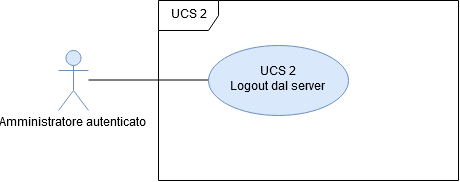
\includegraphics[scale=0.6]{sezioni/UseCase/Immagini/UCS2.png}
  \caption{Logout dal server}
\end{figure}

\begin{itemize}
\item \textbf{Attori primari:} Amministratore autenticato\ap{G};
\item \textbf{Precondizione:} L'amministratore è autenticato\ap{G} presso il server;
\item \textbf{Postcondizione:} L'amministratore non è più autenticato\ap{G} presso il sistema;
\item \textbf{Scenario principale:} L'amministratore seleziona la funzionalità di logout per disconnettersi dal server.
\end{itemize}


% UC... specificare App o Server -> UCA / UCS

%\centering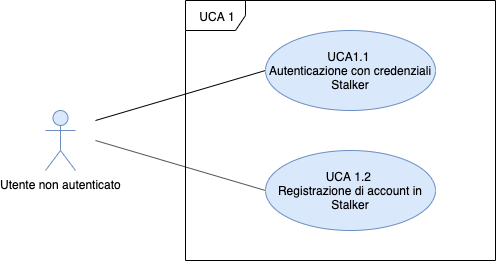
\includegraphics[scale=0.8]{sezioni/UseCase/Immagini/Panoramica.png}
\section{UCS ?}%kite level
\begin{itemize}
    \item \textbf{Nome:} Modifica parametri dell'organizzazione\\
    \item \textbf{Attori primari:} Amministratore gestore\\
    \item \textbf{Precondizione:} L’amministratore dispone di almeno un'organizzazione.\\
    \item \textbf{Postcondizione:} L’amministratore ha modificato i parametri desiderati dell'organizzazione e le modifiche ono state salvate nel sistema.\\
    \item \textbf{Scenario principale:} L'amministratore deve scegliere l'organizzazione che vuole modificare, selezionare la funzionalità di modifica dell'organizzazione e quindi procedere con il cambiamento dei dati.'\\
    \item \textbf{Inclusioni:} UCS Selezione organizzazione
    \item \textbf{Flusso di eventi:}
    \begin{enumerate}
        \item UCS Selezione organizzazione;
        \item L'amministratore ha la possibilità di modificare i campi delle informazioni dell’organizzazione (UCS )
        \item L’amministratore ha la possibilità di modificare il luogo di tracciamento dell’organizzazione [UCS 3.5]
    \end{enumerate}
\end{itemize}
\newpage

\subsubsection{UCS 6 - Selezione del monitoraggio di un'organizzazione o di un luogo specifico}%kite level

\begin{figure}[h]
\centering
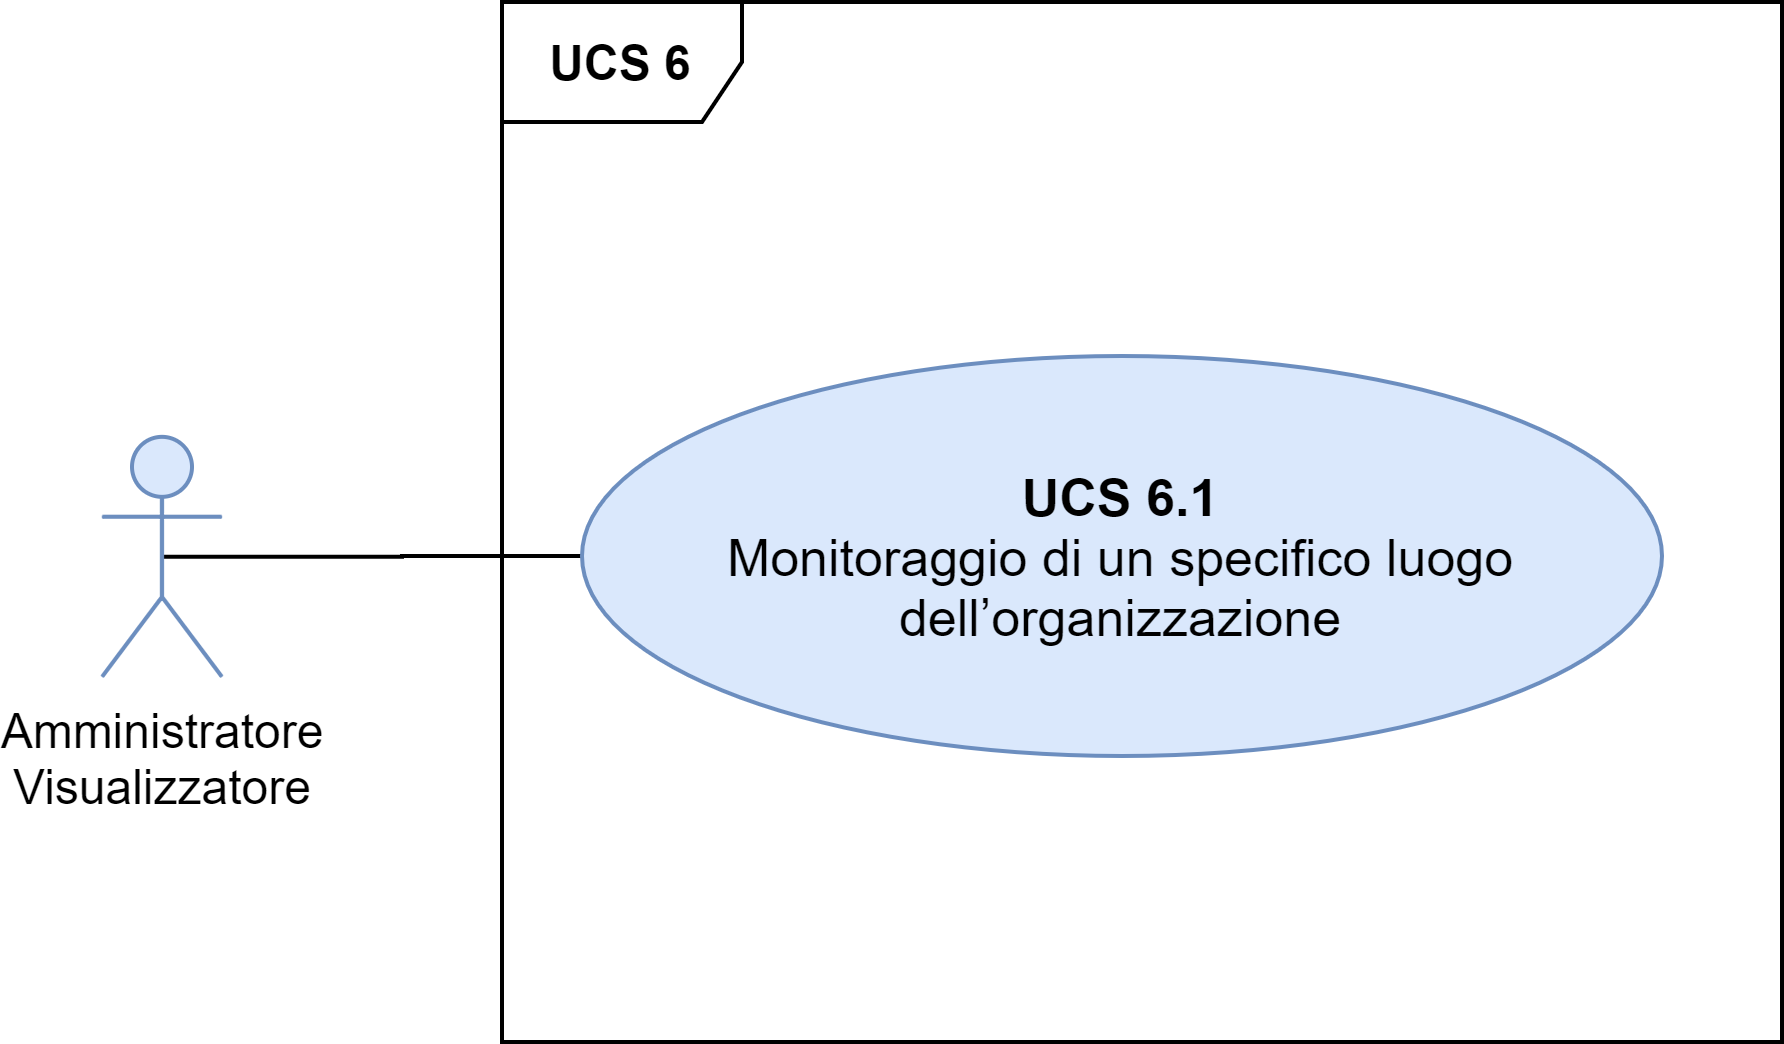
\includegraphics[scale=0.3]{sezioni/UseCase/Immagini/UCS6.png}
\caption{Selezione del monitoraggio di un'organizzazione o di un luogo specifico}
\end{figure}

\begin{itemize}
\item \textbf{Attori primari:} Amministratore visualizzatore;
\item \textbf{Precondizione:} L'amministratore deve essere autenticato\ap{G} presso il sistema;
\item \textbf{Postcondizione:} L'amministratore avrà visualizzato il numero di utenti anonimi presenti in un'organizzazione o in un luogo specifico;
\item \textbf{Scenario principale:} L'amministratore, dopo aver selezionato l'organizzazione, accede alla funzionalità di monitoraggio di un'organizzazione o di un luogo specifico per poter visualizzare il numero di utenti anonimi presenti al suo interno;
\item \textbf{Flusso di eventi:}
\begin{enumerate}
	\item UCS 3 - Selezione dell'organizzazione, oppure UCS 6.4 - Selezione di un luogo specifico;
	\item UCS 6.3 - Selezione della funzionalità di conferma;
	\item UCS 6.1 - Visualizzazione del numero di utenti anonimi di un'organizzazione, oppure UCS 6.2 - Visualizzazione del numero di utenti anonimi di un luogo specifico;
\end{enumerate}
\item \textbf{Estensioni:}  
\begin{enumerate}
	\item Visualizzazione di un messaggio che informa l’indisponibilità del server [?????];
\end{enumerate}
\item \textbf{Inclusioni:}
\begin{enumerate}
	\item UCS 3 - Selezione dell'organizzazione;
\end{enumerate}
\end{itemize}

\subsubsection{UCS 6.1 - Visualizzazione del numero di utenti anonimi di un'organizzazione}%sea level
\begin{itemize}
\item \textbf{Attori primari:} Amministratore visualizzatore;
\item \textbf{Precondizione:} L'amministratore si trova nella sezione di monitoraggio;
\item \textbf{Postcondizione:} L'amministratore ha visualizzato il numero di utenti anonimi contenute nell'organizzazione scelta;
\item \textbf{Scenario principale:} L'amministratore deve aver scelto la funzionalità di conferma per poter visualizzare il numero di utenti anonimi presenti nell'organizzazione scelta;
\item \textbf{Flusso di eventi:} 
\begin{enumerate}
	\item UCS 6.3 - Selezione della funzionalità di conferma;
\end{enumerate}
\item \textbf{Inclusioni:}
\begin{enumerate}
	\item UCS 6.3 - Selezione della funzionalità di conferma.
\end{enumerate}
\end{itemize}

\subsubsection{UCS 6.2 - Visualizzazione del numero di utenti anonimi di un luogo specifico}%sea level
\begin{itemize}
	\item \textbf{Attori primari:} Amministratore visualizzatore;
	\item \textbf{Precondizione:} L'amministratore si trova nella sezione di monitoraggio;
	\item \textbf{Postcondizione:} L'amministratore avrà visualizzato il numero di utenti anonimi contenuto nel luogo specifico presente nell'organizzazione scelta;
	\item \textbf{Scenario principale:} L'amministratore, dopo aver selezionato la funzionalità di monitoraggio di un luogo specifico, sceglierà il luogo specifico che vuole monitorare e successivamente potrà selezionare la funzionalità di conferma che permetterà di visualizzare il numero di utenti anonimi presenti in un luogo specifico;
	\item \textbf{Flusso di eventi:} 
	\begin{enumerate}
		\item UCS 6.4 - Selezione di un luogo specifico;
		\item UCS 6.4.1 - Selezione della funzionalità di monitoraggio di un luogo specifico;
		\item UCS 6.3 - Selezione della funzionalità di conferma;
	\end{enumerate}
	\item \textbf{Inclusioni:}
	\begin{enumerate}
		\item UCS 6.4 - Selezione di un luogo specifico;
		\item UCS 6.3 - Selezione della funzionalità di conferma.
	\end{enumerate}
\end{itemize}

\subsubsection{UCS 6.3 - Selezione della funzionalità di conferma}%sea level
\begin{itemize}
	\item \textbf{Attori primari:} Amministratore visualizzatore;
	\item \textbf{Precondizione:} L'amministratore deve aver selezionato la modalità di monitoraggio del numero di utenti anonimi presenti in un'organizzazione o in un luogo specifico;
	\item \textbf{Postcondizione:} All'amministratore verrà visualizzato il numero di utenti anonimi contenute nell'organizzazione scelta;
	\item \textbf{Scenario principale:} L'amministratore potrà scegliere la funzionalità di conferma che permetterà di visualizzare il numero di utenti anonimi presenti nell'organizzazine scelta o di un suo luogo specifico;
	\item \textbf{Flusso di eventi:} 
	\begin{enumerate}
		\item UCS 6.1 - Visualizzazione del numero di utenti anonimi di un'organizzazione, oppure UCS 6.2 - Visualizzazione del numero di utenti anonimi di un luogo specifico;
	\end{enumerate}
\end{itemize}

\subsubsection{UCS 6.4 - Selezione di un luogo specifico}%sea level
\begin{itemize}
	\item \textbf{Attori primari:} Amministratore visualizzatore;
	\item \textbf{Precondizione:} L'amministratore deve aver selezionato la funzionalità di monitoraggio di un luogo specifico [6.4.1];
	\item \textbf{Postcondizione:} L'amministratore avrà scelto il luogo specifico in cui vuole fare il monitoraggio;
	\item \textbf{Scenario principale:} L'amministratore sceglierà il luogo specifico per poter visualizzare il numero di utenti anonimi presenti che sono all'interno di esso;
	\item \textbf{Flusso di eventi:} 
	\begin{enumerate}
		\item UCS 6.4.1 - Selezione della funzionalità di monitoraggio di un luogo specifico;
	\end{enumerate}
	\item \textbf{Inclusioni:}
	\begin{enumerate}
		\item UCS 6.4.1 - Selezione della funzionalità di monitoraggio di un luogo specifico.
	\end{enumerate}
\end{itemize}

\subsubsection{UCS 6.4.1 - Selezione della funzionalità di monitoraggio di un luogo specifico}
\begin{itemize}
	\item \textbf{Attori primari:} Amministratore visualizzatore;
	\item \textbf{Precondizione:} L'amministratore si trova nella sezione di monitoraggio;
	\item \textbf{Postcondizione:} L'amministratore potrà selezionare il luogo specifico che vuole monitorare.
\end{itemize}




\begin{figure}[h]
\centering
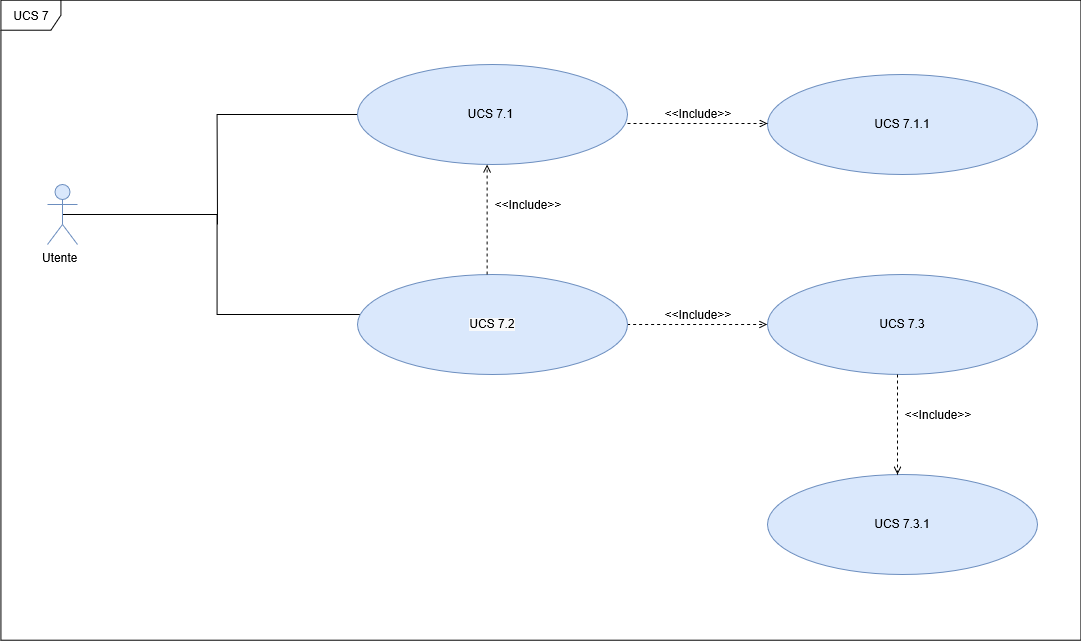
\includegraphics[scale=0.3]{sezioni/UseCase/Immagini/UCS7.png}%location immagine.   immagini/immagine.png
\caption{UCS 7 - Visualizzazione della lista degli accessi di un utente riconosciuto}
\label{logo}
\end{figure}

% UC... specificare App o Server -> UCA / UCS
\section{UCS 7}%kite level
\begin{itemize}
\item \textbf{Nome:} Visualizzazione della lista degli accessi di un utente riconosciuto di un'organizzazione
\item \textbf{Attori primari:} Amministratore visualizzatore
\item \textbf{Precondizione:} L’amministratore deve essere autenticato presso il sistema
\item \textbf{Postcondizione:} L’amministratore avrà visualizzato una lista degli accessi di un utente riconosciuto dell'organizzazione scelta
\item \textbf{Scenario principale:} L’amministratore, dopo aver selezionato l'organizzazione, accede alla funzionalità di visualizzazione della lista degli accessi di un utente riconosciuto e, dopo averlo selezionato, potrà visualizzare la sua lista degli accessi
\item \textbf{Flusso di eventi:} 
\begin{enumerate}
	\item UCS 3 l'amministratore ha selezionato l'organizzazione;
	\item l'amministrazione deve selezionare la funzionalità di visualizzazione della lista degli accessi
\end{enumerate}
\item \textbf{Estensioni:} Visualizzazione di un messaggio che informa l’indisponibilità del server [?????]
\item \textbf{Inclusioni:}
\begin{enumerate}
	\item UCS 3 l'amministratore ha selezionato l'organizzazione;
\end{enumerate}
\end{itemize}

\subsection{UC 7.1}%sea level
\begin{itemize}
\item \textbf{Nome:} Visualizzazione degli accessi di un'utente riconosciuto
\item \textbf{Attori primari:} Amministratore visualizzatore
\item \textbf{Precondizione:} L'amministratore si trova nella sezione di visualizzazione degli accessi di un utente riconosciuto
\item \textbf{Postcondizione:} L'amministratore ha visualizzato una lista con gli accessi di un utente riconosciuto di un'organizzazione
\item \textbf{Scenario principale:} L'amministratore deve aver scelto un'utente riconosciuto, che appartiene all'organizzazione selezionata, per poter visualizzare una sua lista degli accessi
\item \textbf{Flusso di eventi:} 
	\begin{enumerate}
		\item UCS 7.1.1 l'amministratore deve aver scelto l'utente riconosciuto;
	\end{enumerate}
\item \textbf{Inclusioni:}
\begin{enumerate}
	\item UCS 7.1.1;
\end{enumerate}
\end{itemize}

\subsection{UC 7.2}%sea level
\begin{itemize}
	\item \textbf{Nome:} Visualizzazione degli accessi in base a una data di un'utente riconosciuto
	\item \textbf{Attori primari:} Amministratore visualizzatore
	\item \textbf{Precondizione:} L'amministratore si trova nella sezione di visualizzazione degli accessi di un utente riconosciuto
	\item \textbf{Postcondizione:} L'amministratore ha visualizzato una lista con gli accessi di un utente riconosciuto di un'organizzazione che corrispondo alla data inserita dall'amministratore
	\item \textbf{Scenario principale:} L'amministratore deve aver scelto un'utente riconosciuto e, dopo aver aver visualizzato la sua lista degli accessi, può selezionare la funzionalità di selezionamento per data. A questo punto, l'amministratore inserirà una data e verrà visualizzata una lista con tutti gli accessi dell'utente selezionato che corrispondoto a quella data
	\item \textbf{Flusso di eventi:} 
	\begin{enumerate}
		\item UCS 7.1.1 l'amministratore deve aver scelto l'utente riconosciuto;
		\item UCS 7.1 l'amministratore visualizzerà a schermo una lista degli accessi dell'utente riconosciuto selezionato precedentemente;
		\item UCS 7.3.1 l'amministratore deve selezionare la funzionalità di selezione per data;
		\item UCS 7.3 l'amministratore deve inserire una data;
		\item UCS 7.1.1 l'amministratore visualizza gli accessi in base alla data inserita dell'utente riconosciuto scelto;
	\end{enumerate}
	\item \textbf{Inclusioni:}
	\begin{enumerate}
		\item UCS 7.1;
		\item UCS 7.3;
	\end{enumerate}
\end{itemize}

\subsection{UC 7.3}%sea level
\begin{itemize}
	\item \textbf{Nome:} Visualizzazione degli accessi in base a una data di un'utente riconosciuto
	\item \textbf{Attori primari:} Amministratore visualizzatore
	\item \textbf{Precondizione:} L'amministratore deve aver selezionato la funzionalità selezionamento per data (7.3.1)
	\item \textbf{Postcondizione:} L'amministratore avrà inserito la data in cui vuole vedere gli accessi dell'utente riconosciuto
	\item \textbf{Scenario principale:} L'amministratore inserirà una data per poter visualizzare la lista degli accessi dell'utente precedentemente selezionato
	\item \textbf{Flusso di eventi:} 
	\begin{enumerate}
		\item l'amministratore inserisce la data in cui vuole visualizzare gli accessi di un utente riconosciuto;
	\end{enumerate}
	\item \textbf{Inclusioni:}
	\begin{enumerate}
		\item UCS 7.3.1;
	\end{enumerate}
\end{itemize}

\subsubsection{UC 7.3.1}%fish level
\begin{itemize}
\item \textbf{Nome:} Selezione dell'utente riconosciuto
\item \textbf{Attori primari:} Amministratore visualizzatore
\item \textbf{Precondizione:} L'amministratore deve aver visualizzato l'utente riconosciuto 
\item \textbf{Postcondizione:} L'amministratore potrà inserire la data
\end{itemize}

\subsubsection{UC 7.1.1}%fish level
\begin{itemize}
	\item \textbf{Nome:} Selezione della funzionalità di sisualizzazione degli accessi in base a una data 
	\item \textbf{Attori primari:} Amministratore visualizzatore
	\item \textbf{Precondizione:} L'amministratore si trova nella sezione di visualizzazione degli accessi di un utente riconosciuto
	\item \textbf{Postcondizione:} L'amministratore avrà visualizzato l'utente riconosciuto cercato
\end{itemize}




\clearpage

\setcounter{secnumdepth}{3}
\section{Requisiti}
\renewcommand{\o}{Obbligatorio}
\renewcommand{\d}{Desiderabile}
\newcommand{\op}{Opzionale}

Rappresentano dei requisiti che deve soddisfare il prodotto che si vuole realizzare.\\
I requisiti saranno organizzati in forma tabellare.\\
La tabella avrà le seguenti tre colonne:
\begin{itemize}
	\item Codice identificativo
	\item Classificazione
	\item Descrizione
	\item Fonti
\end{itemize}
\paragraph{Codice identificativo dei requisiti}\mbox{}\\
Ogni requisito sarà strutturato come segue:
\begin{itemize}
	\item Identificativo: \textbf{R[Importanza][Tipologia][Codice]}\\
Dove:
\begin{itemize}
		\item \textbf{Importanza:}
		\begin{itemize}
			\item \textbf{1}: requisito obbligatorio, ovvero irrinunciabile per almeno uno degli stakeholder
			\item \textbf{2}: requisito desiderabile, ovvero non strettamente necessario ma che porta valore aggiunto riconoscibile
			\item \textbf{3}: requisito opzionale, ovvero relativamente utile oppure contrattabile più avanti nel progetto
		\end{itemize}
		\item \textbf{Tipologia:}
		\begin{itemize}
			\item \textbf{F}: funzionale, definisce una funzione di un sistema di uno o più dei suoi componenti
			\item \textbf{Q}: qualitativo, definisce un requisito per garantire la qualità per un certo aspetto del progetto
			\item \textbf{P}: prestazionale, definisce un requisito che garantisce efficienza prestazionale nel prodotto
			\item \textbf{V}: vincolo, definisce un requisito volto a far rispettare un dato vincolo
		\end{itemize}
		\item \textbf{Codice:}\\
		Composto da:
		\begin{itemize}
			\item A*\ap{I} se il requisito proviene da un caso d'uso dell'applicazione, dove *\ap{I} sarà composto da: il numero del caso d'uso (lato app) kite-level di provenienza, un punto e il numero progressivo univoco
			\item S*\ap{II} se il requisito proviene da un caso d'uso del server, dove *\ap{II} sarà composto da: il numero del caso d'uso (lato server) kite-level di provenienza, un punto e il numero progressivo univoco
			\item C*\ap{III} se il requisito proviene dal capitolato, dove *\ap{III} sarà il numero progressivo univoco
			\item V*\ap{IV} se il requisito proviene da un verbale, dove *\ap{IV} inizierà con il numero che indica il verbale da cui proviene il requisito; il numero si calcola a partire da 1, che sarà associato al primo verbale redatto (in ordine temporale). Infine vi sarà un punto seguito dal numero progressivo
			\item I*\ap{V} se il requisito proviene da una decisione presa internamente al gruppo, dove *\ap{V} sarà un numero progressivo
		\end{itemize}
\end{itemize}
	\item \textbf{Descrizione}: descrizione sintetica ma al contempo esaustiva del requisito.
	\item \textbf{Classificazione}: informazione ridondante, sotto forma testuale, dell’importanza del requisito. Facilita la lettura dei requisiti.
	\item \textbf{Fonti}: definisce da dove deriva il requisito. I requisiti vengono raccolti da una o più fonti tra quelle citate di seguito:
	\begin{itemize}
		\item \textbf{Capitolato}: requisito individuato dalla lettura e/o analisi del capitolato
		\item \textbf{Interno}: requisito che gli analisti hanno ritenuto opportuno aggiungere
		\item \textbf{Caso d’uso}: il requisito è derivato da uno o più casi d’uso. Riportare anche il/i codice/i identificativo/i del/i caso/i d’uso.
		\item \textbf{Verbale}: requisito derivato in seguito ad una richiesta di chiarimento con il committente. Riportare il nome del documento del verbale da cui deriva il requisito in questione.		
	\end{itemize}
\end{itemize}

\subsection{Requisiti funzionali}
{
\rowcolors{2}{grigetto}{white}
\renewcommand{\arraystretch}{1.5}
\centering
\begin{longtable}{ c C{6.5cm} c c}
\caption{Tabella dei Requisiti funzionali}\\
\rowcolor{darkblue}
\textcolor{white}{\textbf{Identificativo}} & \textcolor{white}{\textbf{Descrizione}} & \textcolor{white}{\textbf{Classificazione}} & \textcolor{white}{\textbf{Fonti}}\\	
\endfirsthead
\rowcolor{darkblue}
\textcolor{white}{\textbf{Identificativo}} & \textcolor{white}{\textbf{Descrizione}} & \textcolor{white}{\textbf{Classificazione}} & \textcolor{white}{\textbf{Fonti}}\\
\endhead

R1FI1 & Un utente non autenticato non può effettuare alcuna azione a meno di autenticazione e registrazione. & \o & Interno\\

R1FA1.1 & L'autenticazione da parte di un utente non autenticato necessita di e-mail. & \o & UCA 1.1.1 Interno\\

R1FA1.2 & L'autenticazione da parte di un utente non autenticato necessita di password. & \o & UCA 1.1.2 Interno\\

R1FA8.1 & L'autenticazione viene negata qualora l'utente non autenticato tenti di autenticarsi con delle credenziali errate. Viene inoltre visualizzato un messaggio d'errore. & \o & UCA 8.1.4 Interno\\

R1FA1.3 & La registrazione da parte di un utente non autenticato necessita di e-mail. & \o & UCA 1.2.1 Interno\\

R1FA8.2 & Il processo di registrazione dell'utente non autenticato viene negato qualora l'e-mail inserita fosse già registrata nel sistema. Viene visualizzato inoltre un messaggio d'errore. & \o & UCA 8.1.1 Interno\\

R1FA1.4 & La registrazione da parte di un utente non autenticato necessita di password. & \o & UCA 1.2.2 Interno\\

R1FA1.5 & La registrazione da parte di un utente non autenticato necessita di conferma della password. & \o & UCA 1.2.3 Interno\\

R1FA1.6 & Durante la registrazione viene chiesto all'utente non autenticato di accettare le condizioni generali d'uso. & \o & UCA 1.2.4 Interno\\

R1FA1.7 & Qualora l'utente non autenticato dovesse rifiutare le condizioni generali d'uso allora la registrazione non può essere terminata correttamente.  & \o & UCA 1.2.4 Interno\\

R2FA1.8 & L'utente non autenticato deve essere in grado di effettuare il reset della password qualora se la fosse dimenticata. & \d & UCA 1.3 Interno\\

R2FA1.9 & Il reset della password da parte dell'utente non autenticato richiede l'e-mail del proprio account. & \d & UCA 1.3.1 Interno\\

R2FA1.10 & Il reset della password da parte dell'utente non autenticato richiede l'e-mail di recupero per effettuare il cambio password. & \d & UCA 1.3.2 Interno\\

R2FA1.11 & Il reset della password da parte dell'utente non autenticato richiede la nuova password. & \d & UCA 1.3.3 Interno\\

R2FA1.12 & Il reset della password da parte dell'utente non autenticato richiede la conferma della nuova password. & \d & UCA 1.3.4 Interno\\

R1FA8.3 & Il processo di autenticazione viene negato qualora la password inserita non sia abbastanza sicura. Viene visualizzato inoltre un messaggio d'errore. & \o & UCA 8.1.2 Interno\\

R1FA8.4 & Il processo di registrazione viene negato se password e conferma password inserita non combaciano. Viene visualizzato inoltre un messaggio d'errore. & \o & UCA 8.1.3 Interno\\


%PERIN

R1FA2.1 & L'utente anonimo e riconosciuto deve essere in grado di effettuare il logout. & \o & UCA 2 Interno\\

R1FA3.1 & L'utente anonimo può gestire la propria lista delle organizzazioni. & \o & UCA 3 Interno\\

R1FA3.2 & L'utente anonimo deve poter essere in grado di scaricare la lista di tutte le organizzazioni. & \o & UCA 3.1 Capitolato \\

R1FA8.5 & Qualora fallisca lo scaricamento della lista delle organizzazioni deve venire visualizzato un messaggio d'errore che lo informa di tale evento. & \o & UCA 8.3.1 Interno \\

R1FA3.3 & L’utente anonimo deve poter essere in grado di gestire la propria lista delle organizzazioni preferite. & \o & UCA 3.2 Interno \\

R1FA3.4 & L’utente anonimo può inserire una organizzazione presente nella lista delle organizzazioni, nella propria lista delle organizzazioni preferite. & \o & UCA 3.2.1 Interno \\

R1FA3.5 & Qualora l’utente anonimo inserisca un'organizzazione nella propria lista delle organizzazioni preferite che richiede autenticazione con credenziali LDAP, deve autenticarsi con credenziali LDAP. & \o & UCA 3.2.2 Capitolato\\

R1FA3.6 & L’utente anonimo può rimuovere una organizzazione presente nella propria lista delle organizzazioni preferite. & \o & UCA 3.2.3 Interno \\

R1FA8.6 & Qualora non sia memorizzata nessuna lista delle organizzazioni nel dispositivo, viene informato l’utente di questo fatto. & \o & UCA 8.3.2 Interno \\

R1FA3.7 & L’utente anonimo ha la possibilità di aggiornare la lista delle organizzazioni. & \o & UCA 3.3 Interno \\

R1FA3.8 & L’utente anonimo può aggiornare la lista delle organizzazioni tramite refresh manuale. & \o & UCA 3.3.1 Interno \\

R1FA3.9 & L’utente  anonimo può aggiornare la lista delle organizzazioni tramite temporizzazione. & \o & UCA 3.3.2 Interno \\

R1FA3.10 & L’utente anonimo può visualizzare la lista delle organizzazioni. & \o & UCA 3.4 Interno \\

R2FA3.11 & L’utente anonimo ha la possibilità di visualizzare la lista delle organizzazioni ordinate alfabeticamente, dalla A alla Z. & \d & UCA 3.4.1 Interno \\

R2FA3.12 & L’utente anonimo ha la possibilità di visualizzare la lista delle organizzazioni ordinate secondo politica \glo{FIFO}. & \d & UCA 3.4.2 Interno \\

R3FA3.13 & L’utente anonimo ha la possibilità di visualizzare la lista delle organizzazioni che permettono il tracciamento anonimo. & \op & UCA 3.4.3 Interno \\

R3FA3.14 & L’utente anonimo ha la possibilità di visualizzare la lista delle organizzazioni che permettono il \glo{tracciamento autenticato}. & \op & UCA 3.4.4 Interno \\

R1FA3.15 & L’utente anonimo può effettuare ricerche personalizzate per cercare le organizzazioni presenti nella lista delle organizzazioni. & \o & UCA 3.5 Interno\\

R2FA3.16 & L’utente anonimo può ricercare organizzazioni presenti nella lista delle organizzazioni appartenenti alla nazione indicata dall’utente. & \d & UCA 3.5.1 Interno \\

R1FA3.17 & L’utente anonimo può ricercare organizzazioni presenti nella lista delle organizzazioni che hanno nel nome una sotto-stringa scelta dall'utente. & \o & UCA 3.5.2 Interno \\

R2FA3.18 & L’utente anonimo può ricercare organizzazioni presenti nella lista delle organizzazioni appartenenti alla città indicata dall’utente. & \d & UCA 3.5.3 Interno \\

R1FA4.1 & L’utente riconosciuto deve poter inserire la modalità di tracciamento che preferisce. & \o & UCA 4 Capitolato \\

R1FA4.2 & L’utente riconosciuto può selezionare la modalità di tracciamento anonimo. & \o & UCA 4.1 Capitolato \\

R1FA4.3 & L’utente riconosciuto può selezionare la modalità di \glo{tracciamento autenticato}. & \o & UCA 4.2 Capitolato \\

R2FA5.1 & L’utente anonimo ha la possibilità di visualizzare il proprio storico degli accessi. & \d & UCA 5 Capitolato \\

R2FA5.2 & L’utente anonimo ha la possibilità di visualizzare il proprio storico degli accessi presso una organizzazione. & \d & UCA 5.1 Capitolato \\

R2FA5.3 & L'utente anonimo nella visualizzazione del proprio storico degli accessi nell'organizzazione visualizza la data per ogni accesso di quando è stato fatto. & \d & UCA 5.1.4 \\

R2FA5.4 & L'utente anonimo nella visualizzazione del proprio storico degli accessi nell'organizzazione visualizza il luogo per ogni accesso di quando è stato fatto. & \d & UCA 5.1.4 \\

R2FA5.5 & L'utente anonimo nella visualizzazione del proprio storico degli accessi nell'organizzazione visualizza il tempo trascorso per ogni accesso. & \d & UCA 5.1.4 \\

R2FA5.6 & L’utente anonimo ha la possibilità di visualizzare il proprio storico degli accessi presso un luogo dell’organizzazione. & \d & UCA 5.2 Capitolato\\

R2FA5.7 & L'utente anonimo nella visualizzazione del proprio storico degli accessi nel luogo dell'organizzazione visualizza la data per ogni accesso di quando è stato fatto. & \d &  UCA 5.2.4 \\

R2FA5.8 & L'utente anonimo nella visualizzazione del proprio storico degli accessi nel luogo dell'organizzazione visualizza il luogo per ogni accesso di quando è stato fatto. & \d &  UCA 5.2.4 \\

R2FA5.9 & L'utente anonimo nella visualizzazione del proprio storico degli accessi nel luogo dell'organizzazione visualizza il tempo trascorso per ogni accesso. & \d &  UCA 5.2.4 \\

R2FA5.10 & L’utente anonimo può visualizzare la propria lista degli accessi in una organizzazione ordinata per data decrescente. & \d & UCA 5.4.1 \\

R2FA5.11 & L’utente anonimo può visualizzare la propria lista degli accessi in una organizzazione ordinata per data crescente. & \d & UCA 5.4.2 \\

R3FA5.12 & L’utente anonimo può effettuare una ricerca degli accessi presso un'organizzazione in un giorno specifico. & \op & UCA 5.5 \\

R2FA5.13 & L’utente anonimo può visualizzare la propria lista degli accessi presso un luogo dell’organizzazione ordinata per data decrescente. & \d & UCA 5.4.1 \\

R2FA5.14 & L’utente anonimo può visualizzare la propria lista degli accessi presso un luogo dell’organizzazione ordinata per data crescente. & \d & UCA 5.4.2 \\

R3FA5.15 & L’utente anonimo può effettuare una ricerca degli accessi presso un luogo dell’organizzazione in un giorno specifico. & \op & UCA 5.5 \\

R2FA5.16 & L’utente anonimo se si trova all’interno dell’organizzazione ha la possibilità di visualizzare il tempo passato all’interno dall'ultimo ingresso effettuato. & \d & UCA 5.1.5 Capitolato \\

R2FA5.17 & L’utente anonimo se si trova all’interno dell’luogo dell’organizzazione ha la possibilità di visualizzare il tempo passato all’interno dall'ultimo ingresso effettuato. & \d & UCA 5.2.5 Capitolato \\

R2FA8.5 & Qualora non ci sono accessi effettuati presso l'organizzazione selezionata, l'utente anonimo deve essere informato di ciò. & \d & UCA 8.5.1 Interno \\

R2FA8.6 & Qualora non ci sono accessi effettuati presso il luogo selezionato, l'utente anonimo deve essere informato di ciò. & \d & UCA 8.5.2 Interno \\

R1FA6.1 & L’utente che effettua un movimento nell’organizzazione deve essere notificato della sua azione e il movimento deve essere memorizzato nel sistema. & \o & UCA 6.1 Capitolato \\

R1FA6.2 & L’utente che effettua un movimento nell’organizzazione, deve essere notificato della sua azione. & \o & UCA 6.1.1 \\

R1FA6.3 & L’utente che effettua un movimento in un luogo all'interno di una organizzazione, deve essere notificato della sua azione. & \o & UCA 6.2.1 \\

R1FA6.4 & L’utente che effettua un movimento in un luogo di un'organizzazione deve essere notificato della sua azione e il movimento deve essere memorizzato nel sistema. & \o & UCA 6.2 Capitolato \\

R1FA8.7 & Qualora non vengano memorizzate le informazioni necessarie per la registrazione del movimento effettuato dall’utente, deve essere notificato tale evento all’utente. & \o & UCA 8.6.1 \\

%Cisotto

R1FA7.1 & L'utente anonimo deve avere la possibilità di autenticarsi con le credenziali aziendali in un'organizzazione che richiede il tracciamento riconosciuto. & \o & UCA 7 Capitolato \\

R1FA8.8 & Qualora le credenziali LDAP aziendali inserite dall'utente non fossero riconosciute dal server aziendale associato viene mostrato un messaggio d'errore. & \o & UCA 8.7.1 Interno \\

R1FA7.2 & L'utente anonimo deve avere la possibilità di inserire il nome utente durante l'autenticazione con le credenziali LDAP aziendali. & \o & UCA 7.1.1 Interno \\

R1FA7.3 & L'utente anonimo deve avere la possibilità di inserire la password durante l'autenticazione con le credenziali LDAP aziendali. & \o & UCA 7.1.2 Interno \\

R1FI2 & Un utente non autenticato non può effettuare alcuna azione a meno di autenticazione. & \o & Interno \\

R1FS1.1 & L’autenticazione da parte di un amministratore necessita di e-mail. & \o & UCS 1.1.1 Interno\\

R1FS10.1 & L’autenticazione viene negata qualora l'amministratore tenti di autenticarsi con delle credenziali errate. & \o & UCS 10.1.1 Interno \\

R1FS10.2 & Qualora l'amministratore tenti di autenticarsi con le credenziali errate viene visualizzato un messaggio d’errore. & \o & UCS 10.1.1 Interno \\

R1FS1.2 & L’autenticazione da parte di un amministratore necessita di password. & \o & UCS 1.1.2 Interno\\

R2FS1.3 & L'utente non autenticato deve essere in grado di effettuare il reset della password qualora se la fosse dimenticata. & \d & UCS 1.3 Interno\\

R2FS1.4 & Il reset della password dell'utente non autenticato richiede l'e-mail. & \d & UCS 1.3.1 Interno \\

R2FS1.5 & Il reset della password dell'utente non autenticato richiede l'e-mail di recupero per il reset della password. & \d & UCS 1.3.2 Interno \\

R2FS1.6 & Il reset della password dell'utente non autenticato richiede la nuova password. & \d & UCS 1.3.3 Interno \\

R2FS1.7 & Il reset della password dell'utente non autenticato richiede la conferma della password. & \d & UCS 1.3.4 Interno \\

R1FS2.1 & L'amministratore deve essere in grado di effettuare il logout. & \o & UCS 2 Interno\\

R1FC3 & L'amministratore visualizzatore deve poter visualizzare le organizzazioni disponibili. & \o & Capitolato\\

R1FI3 & Deve venire mostrato il nome dell'organizzazione durante la sua visualizzazione da parte di un amministratore. & \o & Interno\\

R2FI4 & Deve venire mostrata l'immagine dell'organizzazione durante la sua visualizzazione da parte di un amministratore. & \d & Interno\\

R1FS3.1 & L'amministratore visualizzatore deve poter selezionare un'organizzazione tra quelle da lui visualizzate. & \o & UCS 3 Interno\\

R1FI5 & Deve venire mostrato il nome dell'organizzazione selezionata durante la sua visualizzazione da parte di un amministratore. & \o & Interno\\

R2FI6 & Deve venire mostrata l'immagine dell'organizzazione selezionata durante la sua visualizzazione da parte di un amministratore. & \d & Interno\\

R2FI7 & Deve venire mostrata la descrizione dell'organizzazione selezionata durante la sua visualizzazione da parte di un amministratore. & \d & Interno\\

R1FI8 & Deve venire mostrato l'indirizzo dell'organizzazione selezionata durante la sua visualizzazione da parte di un amministratore. & \o & Interno\\


R1FS4.1 & L'amministratore gestore deve poter modificare il nome dell'organizzazione. & \o & UCS 4.1.1 Interno\\

R2FS4.2 & L'amministratore gestore deve poter modificare l'immagine dell'organizzazione. & \d & UCS 4.1.2 Interno\\

R2FS4.3 & L'amministratore gestore deve poter modificare la descrizione dell'organizzazione. & \d & UCS 4.1.3 Interno\\

R1FS4.4 & L'amministratore gestore deve poter modificare l'indirizzo dell'organizzazione. & \o & UCS 4.1.4 Interno\\

R1FS4.5 & L'amministratore gestore deve poter modificare l'indirizzo IP dell'organizzazione. & \o & UCS 4.1.5 Interno\\

R1FS10.3 & Se il nome dell'organizzazione inserito dall'amministratore non rispetta i vincoli imposti viene mostrato un messaggio d'errore. & \o & UCS 10.4.2\\

R1FS10.4 & Se il nome dell'organizzazione inserito dall'amministratore dovesse essere già presente nel sistema e associato ad un'altra organizzazione viene mostrato un messaggio d'errore. & \o & UCS 10.4.3\\

R2FS10.5 & Se l'immagine dell'organizzazione selezionata dall'amministratore non rispetta i vincoli imposti viene mostrato un messaggio d'errore. & \d & UCS 10.4.4\\

R2FS10.6 & Se la descrizione dell'organizzazione inserita dall'amministratore non rispetta i vincoli imposti viene mostrato un messaggio d'errore. & \d & UCS 10.4.5\\

R1FS10.7 & Se l'indirizzo dell'organizzazione inserito dall'amministratore non rispetta i vincoli imposti viene mostrato un messaggio d'errore. & \o & UCS 10.4.6\\

R1FS10.8 & Se l'indirizzo URL non è valido viene mostrato un messaggio d'errore. & \o & UCS 10.4.7\\

R1FS4.6 & L'amministratore proprietario deve avere la possibilità di inviare la richiesta di eliminazione per un'organizzazione. & \o & UCS 4.2 Capitolato\\

R3FS4.7 & L'amministratore proprietario deve poter inserire una motivazione per la richiesta di eliminazione dell'organizzazione. & \op & UCS 4.2.1 Interno \\

R1FS4.8 & L'amministratore gestore deve poter annullare le modifiche che sta apportando. & \o & UCS 4.3 Interno\\



% Drago

R1FS5.1 & L'amministratore gestore deve poter modificare il perimetro di \glo{tracciamento} dell'\glo{organizzazione}. & \o & UCS 5.1 Capitolato\\

R1FS10.9 & La modifica del perimetro dell'organizzazione viene negata qualora l'amministratore selezioni un area che non rispetta i vincoli imposti. Viene visualizzato un messaggio di errore. & \o & UCS 10.5.1 Capitolato \\

R1FS5.2 & L'amministratore gestore deve essere in grado di creare dei nuovi luoghi di tracciamento nell'organizzazione. & \o & UCS 5.2 Capitolato\\

R1FS5.3 & L'amministratore gestore deve essere in grado di modificare i luoghi di tracciamento dell'organizzazione. & \o & UCS 5.3 Capitolato\\

R1FS10.10 & La creazione di nuovi luoghi e la modifica dell'area di tracciamento di essi vengono negati qualora l'amministratore selezioni un area che fuoriesce dal perimetro. Viene visualizzato un messaggio di errore. & \o & UCS 10.5.2 Capitolato \\

R1FS5.4 & L'amministratore gestore deve essere in grado di eliminare i luoghi di tracciamento dell'organizzazione. & \o & UCS 5.4 Capitolato\\

R1FS5.5 & L'amministratore gestore deve essere in grado di selezionare un'area geografica per il tracciamento del luogo scelto. & \o & UCS 5.5 Capitolato\\

R1FS5.6 & L'amministratore gestore può scegliere l'area di tracciamento tramite l'inserimento delle coordinate geografiche. & \o & UCS 5.5.1 Capitolato\\

R2FS5.7 & L'amministratore gestore può scegliere l'area di tracciamento tramite Google Maps API. & \d & UCS 5.5.2 Interno\\

R1FS5.9 & L'amministratore deve poter inserire un nome per il nuovo luogo di tracciamento. & \o & UCS 5.2.1 Interno\\

R1FS6.1 & L'amministratore può monitorare l'organizzazione visualizzando il numero di utenti anonimi presenti nell'organizzazione. & \o & UCS 6 Capitolato\\

R1FS6.2 & L'amministratore visualizzatore può monitorare l'organizzazione visualizzando il numero di utenti anonimi presenti in un specifico luogo dell'organizzazione. & \o & UCS 6.1 Capitolato\\

R1FS6.3 & L'amministratore visualizzatore ha la possibilità di ritornare al monitoraggio dell'organizzazione in generale dal monitoraggio di un luogo specifico. & \o & UCS 6.1.1 Interno\\

R1FS7.1 & L'amministratore visualizzatore può monitorare gli accessi effettuati dagli utenti riconosciuti. & \o & UCS 7 Capitolato\\

R1FS7.2 & L'amministratore visualizzatore può monitorare gli accessi effettuati presso una organizzazione da un specifico utente riconosciuto visualizzandone il nome, il cognome, l'orario di accesso, di uscita e il tempo di permanenza. & \o & UCS 7.1.4 Capitolato\\

R2FS7.3 & L’amministratore visualizzatore può filtrare la lista degli accessi presso una organizzazione di un utente riconosciuto per data decrescente. & \d & UCS 7.4.1 Interno \\

R2FS7.4 & L’amministratore visualizzatore può filtrare la lista degli accessi presso una organizzazione  di un utente riconosciuto per data crescente. & \d & UCS 7.4.2 Interno \\

R2FS7.5 & L'amministratore visualizzatore può monitorare gli accessi presso una organizzazione filtrandoli in base a una data precisa. & \d & UCS 7.5 Interno\\

R1FS7.6 & L'amministratore visualizzatore può monitorare gli accessi effettuati presso un luogo all'interno di una organizzazione da un specifico utente riconosciuto visualizzandone il nome, il cognome e l'orario di accesso. & \o & UCS 7.2.4 Capitolato\\

R2FS7.7 & L’amministratore visualizzatore può filtrare la lista degli accessi presso un luogo di un'organizzazione di un utente riconosciuto per data decrescente. & \d & UCS 7.4.1 Interno \\

R2FS7.8 & L’amministratore visualizzatore può filtrare la lista degli accessi presso un luogo di un'organizzazione di un utente riconosciuto per data crescente. & \d & UCS 7.4.2 Interno \\

R2FS7.9 & L'amministratore visualizzatore può monitorare gli accessi presso un luogo di un'organizzazione filtrandoli in base a una data precisa. & \d & UCS 7.5 Interno\\

R2FS8.1 & L'amministratore visualizzatore può ricevere un report tabellare degli accessi ai luoghi dell'organizzazione. & \o & UCS 8 Capitolato\\

R2FS8.2 &  Tabella delle entrate e uscite degli utenti nei luoghi dell'organizzazione generabile dall'amministratore visualizzatore di un organizzazione a \glo{tracciamento autenticato}. & \o & UCS 8.1.1 Capitolato\\

R2FS8.3 & Tabella delle ore spese dagli utenti nei luoghi dell'organizzazione generabile dall'amministratore visualizzatore di un organizzazione a \glo{tracciamento autenticato}. & \o & UCS 8.1.2 Capitolato\\

R2FS8.4 & Tabella contenente il numero degli utenti e il totale delle ore passate da essi nei luoghi dell'organizzazione generabile dall'amministratore visualizzatore di un organizzazione a \glo{tracciamento autenticato} o anonimo. & \o & UCS 8.1.3 Capitolato\\

%Cisotto

R1FS9.1 & L'amministratore proprietario ha la possibilità di entrare nella sezione di gestione degli amministratori (per la nomina, eliminazione e modifica dei privilegi ad altri amministratori). & \o & UCS 9 Capitolato \\

R1FI9 & L'amministratore proprietario ha la possibilità di visualizzare gli amministratori da esso nominati una volta entrato nella gestione degli amministratori. & \o & Interno \\

R1FI10 & La visualizzazione di un amministratore deve mostrare la sua e-mail. & \o & Interno \\

R1FI11 & La visualizzazione di un amministratore deve mostrare i suoi privilegi. & \o & Interno \\

R1FS9.2 & L'amministratore proprietario ha la possibilità di nominare un nuovo amministratore. & \o & UCS 9.1 Capitolato\\

R1FS9.3 & L'amministratore proprietario deve poter inserire un'e-mail per il nuovo amministratore da nominare. & \o & UCS 9.1.1 Interno\\

R1FS10.11 & Viene mostrato un messaggio d'errore qualora l'e-mail del nuovo amministratore da nominare risulti già registrata nel sistema. & \o & UCS 10.9.1 Interno\\

R1FS10.12 & Viene mostrato un messaggio d'errore qualora la password del nuovo amministratore da nominare risulti troppo debole. & \o & UCS 10.9.2 Interno\\

R1FS10.13 & Viene mostrato un messaggio d'errore qualora la password non combaci con la conferma password del nuovo amministratore da nominare. & \o & UCS 10.9.3 Interno\\

R1FS9.4 & L'amministratore proprietario deve poter inserire una nuova password per il nuovo amministratore da nominare. & \o & UCS 9.1.2 Interno\\

R1FS9.5 & L'amministratore proprietario deve poter inserire la conferma della nuova password per il nuovo amministratore da nominare. & \o & UCS 9.1.3 Interno\\

R1FS9.6 & L'amministratore proprietario deve poter selezionare i privilegi per il nuovo amministratore da nominare. & \o & UCS 9.1.4 Interno\\

R1FS9.7 & L'amministratore proprietario ha la possibilità di eliminare un amministratore togliendogli i permessi di amministrazione dell'organizzazione. & \o & UCS 9.2 Capitolato\\

R1FS9.8 & L'amministratore proprietario ha la possibilità di inserire la e-mail dell'account amministratore da eliminare. & \o & UCS 9.2.1 Interno\\

R1FS10.14 & Viene mostrato un messaggio d'errore qualora l'e-mail dell'amministratore da eliminare inserita non risulti registrata nel sistema. & \o & UCS 10.9.4 Interno\\

R1FS9.9 & L'amministratore proprietario ha la possibilità di modificare i privilegi di un amministratore. & \o & UCS 9.3 Interno\\

R1FS9.10 & L'amministratore proprietario ha la possibilità di inserire la e-mail dell'account amministratore a cui desidera modificare i privilegi. & \o & UCS 9.3.1 Interno\\

R1FS10.15 & Viene mostrato un messaggio d'errore qualora l'e-mail dell'amministratore a cui si vuole modificare i privilegi non risulti registrata nel sistema. & \o & UCS 10.9.4 Interno\\

R1FS9.11 & L'amministratore proprietario ha la possibilità annullare le modifiche che sta apportando agli amministratori. & \o & UCS 9.4 Interno\\

R1FS9.12 & L'amministratore proprietario ha la possibilità di nominare un account già presente nel sistema come amministratore della propria organizzazione & \o & UCS 9.5 Interno\\

R1FS9.13 & L'amministratore proprietario deve poter inserire un'e-mail per il nuovo amministratore da nominare. & \o & UCS 9.5.1 Interno\\

R1FS9.14 & L'amministratore proprietario deve poter selezionare i privilegi per il nuovo amministratore da nominare. & \o & UCS 9.5.2 Interno\\

R1FS10.16 & L'amministratore gestore deve poter annullare le modifiche che stava apportando all'organizzazione. & \o & UCS 10.4.1\\

R1FS10.17 & L'amministratore gestore deve poter annullare la selezione della nuova area geografica per il tracciamento di un luogo o del perimetro dell'organizzazione. & \o & UCS 10.5.3 Interno\\

R2FS10.18 & Deve venir mostrato un errore qualora avvenisse un errore da parte del server sulla generazione del report tabellare. & \d & UCS 10.6.1 Interno\\

\end{longtable}
}
\subsection{Requisiti prestazionali}
{
\rowcolors{2}{grigetto}{white}
\renewcommand{\arraystretch}{1.5}
\centering
\begin{longtable}{ c C{8cm} c c}
\rowcolor{rossoep}
\textcolor{white}{\textbf{Identificativo}} & \textcolor{white}{\textbf{Descrizione}} & \textcolor{white}{\textbf{Classificazione}} & \textcolor{white}{\textbf{Fonti}}\\	
\endhead

R1PC1 & L'applicazione deve bilanciare nel miglior modo possibile il consumo della batteria & Obbligatorio & Capitolato\\

R1PC2 & Il rintracciamento deve avere una precisione sufficiente a certificare la presenza della persona all'interno degli edifici & Obbligatorio & Capitolato\\

%R1PC3 & Scalabilità orizzontale?? & Obbligatorio & Capitolato\\
\end{longtable}
}
\subsection{Requisiti qualitativi}
{
\rowcolors{2}{grigetto}{white}
\renewcommand{\arraystretch}{1.5}
\centering
\begin{longtable}{ c C{8cm} c c}
\rowcolor{darkblue}
\textcolor{white}{\textbf{Identificativo}} & \textcolor{white}{\textbf{Descrizione}} & \textcolor{white}{\textbf{Classificazione}} & \textcolor{white}{\textbf{Fonti}}\\	
\endhead

R1QI1 & Le norme e le metriche definite nei documenti \textit{NormeDiProgetto} e \textit{PianoDiQualifica} sono state rispettate. & Obbligatorio & Interno\\

R1QI2 & Deve essere prodotto un manuale utente. & Obbligatorio & Interno\\

R1QI3 & Deve essere prodotto un manuale amministratore. & Obbligatorio & Interno\\

R1QI4 & Il codice sorgente deve essere caricato in una repository su GitHub. & Obbligatorio & Interno\\

R1QI5 & La documentazione riguardante il software deve essere disponibile in lingua italiana. & Obbligatorio & Interno\\

R1QV1 & Si deve scegliere una licenza tra GNU\ap{G}, GPL\ap{G}, LGPL\ap{G} e MIT\ap{G}. & Obbligatorio & VE\_2019\_12\_16 \\

\end{longtable}
}
\renewcommand{\o}{Obbligatorio}
\renewcommand{\d}{Desiderabile}
\subsection{Requisiti di vincolo}
{
\rowcolors{2}{grigetto}{white}
\renewcommand{\arraystretch}{2}
\centering
\begin{longtable}{ c C{8cm} c c}
\rowcolor{darkblue}
\textcolor{white}{\textbf{Identificativo}} & \textcolor{white}{\textbf{Descrizione}} & \textcolor{white}{\textbf{Classificazione}} & \textcolor{white}{\textbf{Fonti}}\\	
\endhead

R1VC1.1 & Deve essere sviluppato un server back-end & \o & Capitolato \\
R1VC1.2 & Il server deve essere correlato di una UI\ap{G} per la gestione delle funzioni implementate& \o & Capitolato \\
R1VC1.3 & Deve essere sviluppata una applicazione mobile per sistemi operativi Android o IOS & \o & Capitolato \\
R1VC2.1 & Le comunicazioni di tracciamento tra applicazione cellulare e Server devono avvenire solo al momento d’ingresso ed uscita dai luoghi designati & \o & Capitolato \\
R2VC3.1 & Possibile utilizzo di Java\ap{G} (versioni 8 o superiori) per sviluppo Server back-end & \d & Capitolato \\
R2VC3.2 & Possibile utilizzo di Python\ap{G} per sviluppo server back-end & \d & Capitolato \\
R2VC3.3 & Possibile utilizzo di Nodejs\ap{G}per sviluppo server back-end & \d & Capitolato \\
R2VC4.1 & Possibile utilizzo di protocolli asincroni\ap{G} per le comunicazioni app mobile-server & Desiderato & Capitolato \\
R2VC5.1 & Possibile utilizzo del pattern di Publish/Subscriber\ap{G} & \d & Capitolato \\
R2VC6.1 & Possibile utilizzo dell’IAAS Kubernetes\ap{G} per la gestione della scalabilità orizzontale\ap{G}& \d & Capitolato \\
R2VC6.2 & Possibile utilizzo di PAAS\ap{G} per la gestione della scalabilità orizzontale\ap{G}& \d & Capitolato \\
R2VC6.3 & Possibile utilizzo di Openshift\ap{G} per la gestione della scalabilità orizzontale\ap{G}& \d & Capitolato \\
R2VC6.4 & Possibile utilizzo di Rancher\ap{G} per la gestione della scalabilità orizzontale\ap{G}& \d & Capitolato \\
R1VC7.1 & Il server deve esporre oltre a eventuali protocolli richiesti per l’interazione con il servizio, delle API Rest\ap{G} necessarie per permettere l’utilizzo applicativo, come alternativa alle API Rest\ap{G} è possibile utilizzare gRPC\ap{G} & \o & Capitolato \\
R2VC8.1 & Utilizzo di tecnologie network-GPS\ap{G} per il tracciamento della posizione & \d & Capitolato \\
R1VC8.2 & Si deve fornire un resoconto sulle scelte fatte e sui test effettuati relativi al tracciamento della posizione & \o & Capitolato \\
R1VC9.1 & Si deve correlare a tutte le componenti applicative dei test di unità e d’integrazione & \o & Capitolato \\
R1VC9.2 & Si deve testare tramite test end to end il sistema nella sua interezza & \o & Capitolato \\
R1VC9.3 & Devono essere effettuati test di carico per testare il corretto funzionamento della scalabilità & \o & Capitolato \\
R1VC9.4 & Si deve avere una copertura dei test maggiore o uguale al 80\% & \o & Capitolato \\
R1VC9.5 & Tutti i test effettuati devono essere correlati da un report & \o & Capitolato \\
R1VC10.1 & Deve essere scritta la documentazione relativa alle scelte implementative e progettuali con annessa motivazione & \o & Capitolato \\
R1VC10.2 & Deve essere scritta la documentazione relativa ai problemi aperti e eventuali soluzioni proposte da esplorare & \o & Capitolato \\
R2VC11.1 & Cifratura di tutte le comunicazioni fra App e Server & \d & Capitolato  \\
R1VC12.1 & Si deve utilizzare il protocollo LDAP per autenticare i singoli dipendenti e gli amministratori di una organizzazione per poter effettuare il tracciamento autenticato della posizione & \o & Capitolato \\	
R1VV1.1 & Deve essere garantita la privacy e quindi verificare che tutte le informazioni raccolte rispettino le GDPR\ap{G} & \o & VE\_2019\_12\_16 \\
R1VV1.2 & Le credenziali per accedere alla applicazione e le credenziali per accedere e autenticarsi in una organizzazione che richiede tracciamento autenticato devono essere diverse & \o & VE\_2019\_12\_16 \\
R1VV1.3 & I server LDAP delle organizzazioni che richiedono autenticazione devono essere esterni al sistema.  & \o & VE\_2019\_12\_16 \\
R1VV1.4 & Per gli utenti che non devono essere autenticati, si deve assegnare a loro un codice che ne certifichi la validità dell’ingresso o dell'uscita da un luogo in modo tale da non conoscere chi lo ha generato & \o & VE\_2019\_12\_16 \\
\end{longtable}
}

\section{Tracciamento}
\subsection{Tracciamento Fonte-Requisito}
{
\rowcolors{2}{grigetto}{white}
\renewcommand{\arraystretch}{1.5}
\centering
\begin{longtable}{ c C{4cm} c c}
\rowcolor{rossoep}
\textcolor{white}{\textbf{Fonte}} & \textcolor{white}{\textbf{Requisito}}\\	
\endhead

%% Requisiti funzionali

Interno & R1FI1\\

Interno & R1FA1.1\\

Interno & R1FA1.2\\

Interno & R1FA8.1\\

Interno & R1FA1.3\\

Interno & R1FA8.2\\

Interno & R1FA1.4\\

Interno & R1FA1.5\\

Interno & R1FA1.6\\

Interno & R1FA1.7\\

%%SEPARAZIONE

Interno & R2FA1.8\\

Interno & R1FA8.3\\

Interno & R1FA8.4\\

Interno & R1FA2\\

Interno & R1FA3.1\\

Capitolato & R1FA3.2\\

Interno & R1FA8.3\\

Interno & R1FA3.3\\

Interno & R1FA3.4\\

%% SEPARAZIONE

Capitolato & R1FA3.5\\

Interno & R1FA3.6\\

Interno & R1FA8.4\\

Interno & R1FA3.7\\

Interno & R1FA3.8\\

Interno & R1FA3.9\\

Interno & R1FA3.10\\

Interno & R1FA3.11\\

Interno & R1FA3.12\\

Interno & R1FA3.13\\

%% SEPARAZIONE

Interno & R1FA3.14\\

Interno & R1FA3.15\\

Interno & R1FA3.16\\

Interno & R1FA3.17\\

Interno & R1FA3.18\\

Capitolato & R1FA4.1\\

Capitolato & R1FA4.2\\

Capitolato & R1FA4.3\\

Capitolato & R2FA5.1\\

Capitolato & R2FA5.2\\

%% SEPARAZIONE

Interno & R2FA5.3\\

Interno & R2FA5.4\\

Interno & R2FA5.5\\

Capitolato & R2FA5.6\\

Interno & R2FA5.7\\

Interno & R2FA5.8\\

Interno & R2FA5.9\\

Interno & R2FA5.10\\

Interno & R2FA5.11\\

%% SEPARAZIONE

Interno & R2FA5.12\\

Interno & R2FA5.13\\

Interno & R2FA5.14\\

Interno & R3FA5.15\\

Capitolato & R2FA5.16\\

Capitolato & R2FA5.17\\

Interno & R2FA8.5\\

Interno & R2FA8.6\\

Capitolato & R2FA6.1\\

%% SEPARAZIONE

Interno & R2FA6.2\\

Interno & R2FA6.3\\

Interno & R2FA6.4\\

Capitolato & R2FA6.5\\

Capitolato & R2FA6.6\\

Capitolato & R2FA6.7\\

Capitolato & R2FA6.8\\

%% SEPARATORE

Interno & R2FA8.7\\

Interno & R2FA6.9\\

Capitolato & R1F7.1\\

Interno & R1F8.8\\

Interno & R1F7.2\\

Interno & R1F7.3\\

Interno & R1FI2\\

Interno & R1FS1.1\\

Interno & R1FS10.1\\

%% SEPARATORE

Interno & R1FS10.2\\

Interno & R1FS1.2\\

Interno & R2FS1.3\\

Interno & R1FS2.1\\

Capitolato & R1FC3\\

Interno & R1FI3\\

Interno & R2FI4\\

Interno & R1FS3.1\\

Interno & R1FI5\\

Interno & R2FI6\\

Interno & R2FI7\\

%% SEPARATORE

Interno & R1FI8\\

Interno & R1FS4.1\\

Interno & R1FS4.2\\

Interno & R2FS4.3\\

Interno & R2FS4.4\\

Interno & R2FS4.5\\

Interno & R2FS4.6\\

Interno & R1FS4.7\\

Interno & R1FS4.8\\

Interno & R1FS4.9\\

Interno & R1FS4.10\\

%% SEPARATORE

Interno & R1FS10.3\\

Interno & R1FS10.4\\

Interno & R2FS10.5\\

Interno & R2FS10.6\\

Interno & R1FS10.7\\

Interno & R1FS10.8\\

Capitolato & R1FS4.9\\

%% SEPARATORE

Interno & R3FS4.10\\

Interno & R1FS4.11\\

Capitolato & R1FS5.1\\

Capitolato & R1FA10.9\\

Capitolato & R1FS5.2\\

Capitolato & R1FS5.3\\

Capitolato & R1FS10.10\\

Capitolato & R1FS5.4\\

Capitolato & R1FS5.5\\

%% SEPARATORE

Capitolato & R1FS5.6\\

Interno & R2FS5.7\\

Interno & R1FS5.8\\

Capitolato & R1FS6.1\\

Capitolato & R1FS6.2\\

Capitolato & R1FS7.1\\

Capitolato & R1FS7.2\\

Interno & R2FS7.3\\

Interno & R2FS7.4\\

Interno & R2FS7.5\\

Capitolato & R1FS7.6\\

Capitolato & R1FS8.1\\

%% SEPARATORE

Capitolato & R1FS8.2\\

Capitolato & R1FS8.3\\

Capitolato & R1FS8.4\\

Capitolato & R1FS9.1\\

Interno & R1FI9\\

Interno & R1FI10\\

Interno & R1FI11\\

Capitolato & R1FS9.2\\

%% SEPARATORE

Interno & R1FS9.3\\

Interno & R1FS10.11\\

Interno & R1FS10.12\\

Interno & R1FS10.13\\

Interno & R1FS9.4\\

Interno & R1FS9.5\\

Interno & R1FS9.6\\

Capitolato & R1FS9.7\\

Interno & R1FS9.8\\

%% SEPARATORE

Interno & R1FS10.14\\

Interno & R1FS9.9\\

Interno & R1FS9.10\\

Interno & R1FS10.15\\

Interno & R1FS9.11\\

%% Requisiti funzionali

Capitolato & R1PC1\\

Capitolato & R1PC2\\

%% Requisiti qualitativi

Interno & R1QI1\\

Interno & R1QI2\\

Interno & R1QI3\\

Interno & R1QI4\\

Interno & R1QI5\\

VE\_2019\_12\_16 & R1QVE1\\

%% Requisiti di vincolo

Capitolato & R1VC1.1\\

Capitolato & R1VC1.2\\

Capitolato & R1VC1.3\\

Capitolato & R1VC2.1\\

Capitolato & R2VC3.1\\

Capitolato & R2VC3.2\\

Capitolato & R2VC3.3\\

Capitolato & R2VC4.1\\

Capitolato & R2VC5.1\\

%% SEPARATORE

Capitolato & R2VC6.1\\

Capitolato & R2VC6.2\\

Capitolato & R2VC6.3\\

Capitolato & R2VC6.4\\

Capitolato & R1VC7.1\\

Capitolato & R2VC8.1\\

Capitolato & R2VC8.2\\

Capitolato & R1VC9.1\\

Capitolato & R1VC9.2\\

Capitolato & R1VC9.3\\

Capitolato & R1VC9.4\\

Capitolato & R1VC9.5\\

Capitolato & R1VC10.1\\

Capitolato & R1VC10.2\\

Capitolato & R2VC11.1\\

Capitolato & R2VC12.1\\

%% SEPARATORE

VE\_2019\_12\_16 & R1VV1.1\\

VE\_2019\_12\_16 & R1VV1.2\\

VE\_2019\_12\_16 & R1VV1.3\\

VE\_2019\_12\_16 & R1VV1.4\\


\end{longtable}
}


\subsection{Tracciamento Caso d'uso-Requisito}
{
\rowcolors{2}{grigetto}{white}
\renewcommand{\arraystretch}{1.5}
\centering
\begin{longtable}{ c C{4cm} c c}
\rowcolor{rossoep}
\textcolor{white}{\textbf{Caso d'uso}} & \textcolor{white}{\textbf{Requisito}}\\	
\endhead

%% Requisiti funzionali

UCA 1.1.1 & R1FA1.1\\

UCA 1.1.2 & R1FA1.2\\

UCA 7 & R1FA7.1\\

UCA 1.2.1 & R1FA1.3\\

UCA 7.1.1 & R1FA7.2\\

UCA 1.2.2 & R1FA1.4\\

UCA 1.2.3 & R1FA1.5\\

UCA 1.2.4 & R1FA1.6\\

UCA 1.2.4 & R1FA1.7\\

%%SEPARAZIONE

UCA 1.3 & R2FA1.8\\

UCA 8.1.3 & R1FA8.3\\

UCA 8.1.3 & R1FA8.4\\

UCA 2 & R1FA2\\

UCA 3 & R1FA3.1\\

UCA 3.1 & R1FA3.2\\

UCA 8.1.3 & R1FA8.3\\

UCA 3.2 & R1FA3.3\\

UCA 3.2.1 & R1FA3.4\\

%% SEPARAZIONE

UCA 3.2.2 & R1FA3.5\\

UCA 3.2.3 & R1FA3.6\\

UCA 8.1.3 & R1FA8.4\\

UCA 3.3 & R1FA3.7\\

UCA 3.3.1 & R1FA3.8\\

UCA 3.3.2 & R1FA3.9\\

UCA 3.4 & R1FA3.10\\

UCA 3.4.1 & R1FA3.11\\

UCA 3.4.2 & R1FA3.12\\

UCA 3.4.3 & R1FA3.13\\

%% SEPARAZIONE

UCA 3.4.4 & R1FA3.14\\

UCA 3.5 & R1FA3.15\\

UCA 3.5.1 & R1FA3.16\\

UCA 3.5.2 & R1FA3.17\\

UCA 3.5.3 & R1FA3.18\\

UCA 4 & R1FA4.1\\

UCA 4.1 & R1FA4.2\\

UCA 4.2 & R1FA4.3\\

UCA 5 & R2FA5.1\\

UCA 5.1 & R2FA5.2\\

%% SEPARAZIONE

UCA 5.1 & R2FA5.3\\

UCA 5.1 & R2FA5.4\\

UCA 5.1 & R2FA5.5\\

UCA 5.2 & R2FA5.6\\

UCA 5.1 & R2FA5.7\\

UCA 5.1 & R2FA5.8\\

UCA 5.1 & R2FA5.9\\

UCA 5.1.1 & R2FA5.10\\

UCA 5.1.2 & R2FA5.11\\

%% SEPARAZIONE

UCA 5.1.3 & R2FA5.12\\

UCA 5.2.1 & R2FA5.13\\

UCA 5.2.2 & R2FA5.14\\

UCA 5.2.3 & R3FA5.15\\

UCA 5.1 & R2FA5.16\\

UCA 5.2 & R2FA5.17\\

UCA 8.5.1 & R2FA8.5\\

UCA 8.5.2 & R2FA8.6\\

UCA 6 & R2FA6.1\\

%% SEPARAZIONE

UCA 6.1.1 & R2FA6.2\\

UCA 6.1.1 & R2FA6.3\\

UCA 6 & R2FA6.4\\

UCA 6.1 & R2FA6.5\\

UCA 6.2 & R2FA6.6\\

UCA 6.3 & R2FA6.7\\

UCA 6.4 & R2FA6.8\\

%% SEPARATORE

UCA 8.6.1 & R2FA8.7\\

UCA 6.1.3 & R2FA6.9\\

UCA 7 & R1FA7.1\\

UCA 8.7.1 & R1FA8.8\\

UCA 7.1.1 & R1FA7.2\\

UCA 7.1.2 & R1FA7.3\\

UCS 1.1.1 & R1FS1.1\\

UCS 10.1.1 & R1FS10.1\\

%% SEPARATORE

UCS 10.1.1 & R1FS10.2\\

UCS 1.1.2 & R1FS1.2\\

UCS 1.3 & R2FS1.3\\

UCS 2 & R1FS2.1\\

UCS 3 & R1FS3.1\\

%% SEPARATORE

UCS 4.1.1 & R1FS4.1\\

UCS 4.1.1 & R1FS4.2\\

UCS 4.1.2 & R2FS4.3\\

UCS 4.1.2 & R2FS4.4\\

UCS 4.1.3 & R2FS4.5\\

UCS 4.1.3 & R2FS4.6\\

UCS 4.1.4 & R1FS4.7\\

UCS 4.1.4 & R1FS4.8\\

UCS 4.1.5 & R1FS4.9\\

UCS 4.1.5 & R1FS4.10\\

%% SEPARATORE

UCS 10.4.2 & R1FS10.3\\

UCS 10.4.3 & R1FS10.4\\

UCS 10.4.4 & R2FS10.5\\

UCS 10.4.5 & R2FS10.6\\

UCS 10.4.6 & R1FS10.7\\

UCS 10.4.7 & R1FS10.8\\

UCS 4.2 & R1FS4.9\\

%% SEPARATORE

UCS 4.2.1 & R3FS4.10\\

UCS 4.3 & R1FS4.11\\

UCS 5.1 & R1FS5.1\\

UCS 10.5.1 & R1FA10.9\\

UCS 5.2 & R1FS5.2\\

UCS 5.3 & R1FS5.3\\

UCS 10.5.2 & R1FS10.10\\

UCS 5.4 & R1FS5.4\\

UCS 5.5 & R1FS5.5\\

%% SEPARATORE

UCS 5.5.1 & R1FS5.6\\

UCS 5.5.2 & R2FS5.7\\

UCS 5.5.3 & R1FS5.8\\

UCS 6 & R1FS6.1\\

UCS 6.1 & R1FS6.2\\

UCS 7 & R1FS7.1\\

UCS 7.1 & R1FS7.2\\

UCS 7.1.1 & R2FS7.3\\

UCS 7.1.2 & R2FS7.4\\

UCS 7.1.3 & R2FS7.5\\

UCS 7.2 & R1FS7.6\\

UCS 8 & R1FS8.1\\

%% SEPARATORE

UCS 8.1.1 & R1FS8.2\\

UCS 8.1.2 & R1FS8.3\\

UCS 8.1.3 & R1FS8.4\\

UCS 9 & R1FS9.1\\

UCS 9.1 & R1FS9.2\\

%% SEPARATORE

UCS 9.1.1 & R1FS9.3\\

UCS 10.9.1 & R1FS10.11\\

UCS 10.9.2 & R1FS10.12\\

UCS 10.9.3 & R1FS10.13\\

UCS 9.1.2 & R1FS9.4\\

UCS 9.1.3 & R1FS9.5\\

UCS 9.1.4 & R1FS9.6\\

UCS 9.2 & R1FS9.7\\

UCS 9.2.1 & R1FS9.8\\

%% SEPARATORE

UCS 10.9.4 & R1FS10.14\\

UCS 9.3 & R1FS9.9\\

UCS 9.3.1 & R1FS9.10\\

UCS 10.9.4 & R1FS10.15\\

UCS 9.4 & R1FS9.11\\

\end{longtable}
}

























\end{document}

\subsubsection{Progettazione}
\paragraph{Scopo}\mbox{}\\ \\
La progettazione, svolta dai Progettisti, ha lo scopo di soddisfare i requisiti stabiliti nel documento \AdR{} per trovare una soluzione accettabile per tutti gli stakeholder.
Per fare ciò, si cerca di seguire un approccio sintetico dove si pensa prima all’architettura del prodotto e poi al codice.
\paragraph{Descrizione}\mbox{}\\ \\
La progettazione consiste nei seguenti compiti:
\begin{itemize}
	\item Controllare la complessità del prodotto suddividendo il sistema in parti di complessità trattabile;
	\item Soddisfare i requisiti garantendo qualità;
	\item Definire un’architettura logica del prodotto che dovrà avere determinate caratteristiche;
	\item Avere una progettazione dettagliata con la consapevolezza di fermarsi quando la suddivisione porterà più svantaggi che benefici.
\end{itemize}

\paragraph{Architettura}\mbox{}\\ \\
I progettisti devono definire l’architettura logica del prodotto creando parti con specifiche chiare, coese e realizzabili con risorse sostenibili e mantenibili. L'architettura deve avere determinate caratteristiche per:
\begin{itemize}
	\item Soddisfare tutti requisiti degli stakeholder;
	\item Riuscire a gestire gli errori quando presenti;
	\item Garantire che venga eseguito il suo compito nel modo corretto;
	\item Cercare di ridurre i tempi di manutenzione;
	\item Avere componenti semplici, coesi, incapsulati e di basso accoppiamento tra di loro.
\end{itemize}

La realizzazione dell’architettura del prodotto è divisa in due parti:
\begin{itemize}
	\item Technology Baseline\ap{G};
	\item Product Baseline\ap{G}.
\end{itemize}

\subparagraph{Technology Baseline}\mbox{}\\ \\
La Technology Baseline deve dimostrare l’adeguatezza dell’architettura tramite un Proof of Concept (PoC) che rappresenta la baseline per lo sviluppo. 
La Technology baseline deve includere:
\begin{itemize}
	\item Le tecnologie;
	\item I framework;
	\item Le librerie utilizzate nel Proof of Concept;
	\item Diagrammi UML con le seguenti rappresentazioni:
	\begin{itemize}
		\item Diagrammi dei casi d'uso; 
		\item Diagrammi delle classi; 
		\item Diagrammi dei package;
		\item Diagrammi di sequenza; 
		\item Diagrammi di attività.
	\end{itemize}
\end{itemize}

\subparagraph{Product Baseline}\mbox{}\\ \\
La Product Baseline illustrerà la baseline architetturale del prodotto, in coerenza con la Technology Baseline.
Essa deve includere un allegato che contenga:
\begin{itemize}
	\item Diagrammi delle classi;
	\item Diagrammi di sequenza;
	\item Contestualizzazione dei design pattern adottati.	
\end{itemize}

\documentclass[a4paper, oneside, dvipsnames, table]{article}
\usepackage{hyperref}
\usepackage{fancyhdr}
\usepackage[italian]{babel}
\usepackage[raggedright]{titlesec}
\usepackage{blindtext}
\titleformat{\paragraph}[hang]{\normalfont\normalsize\bfseries}{\theparagraph}{1em}{}
\titlespacing*{\paragraph}{0pt}{3.25ex plus 1ex minus .2ex}{0.5em}


\begin{document}

\subsection{Codifica}

Questa sezione è stata fatta durante la fase iniziale del progetto e di conseguenza verrà ampliata in seguito durante la fase di \textbf{Programmazione}.
%%SCRIVERE MEGLIO
Lo scopo di questa sezione è di descrivere le norme che i programmatori dovranno rispettare durante tutto il ciclo di vita del software. 

\subsubsection{Commenti}
I commenti devono essere i più sintetici meno invasivi possibili.
Ogni volta che verrà scritto un nuovo frammento di codice i commenti dovranno essere usati per:
\begin{itemize}
\item Identificare chi ha scritto il frammento di codice;
\item Descrivere cosa fa il frammento di codice.
\end{itemize}

\subsubsection{Nomi}
\begin{itemize}
\item I nomi devono essere univoci;
\item I nomi devono essere chiari e descrittivi;
\item I nomi non devono essere simili fra di loro, per evitare confusione;
\item I nomi formati da più parole si devono scrivere usando l'underscore come separatore o, in alternativa, separare i termini con una lettera maiuscola.
\end{itemize}

\end{document}